%%%%%%%%%%%%%%%%%%%%%%%%%%%%%%%%%%%%%%%%%%%%%%%%%%%%%%%%%%%%%%%%%%%%%%%%%%%%%%%%
%%%%%%%%%%%%%%%%%%%%%%%%%%%%%%%%%%%%%%%%%%%%%%%%%%%%%%%%%%%%%%%%%%%%%%%%%%%%%%%%
%%                                                                            %%
%% thesistemplate.tex version 3.20 (2018/08/31)                               %%
%% The LaTeX template file to be used with the aaltothesis.sty (version 3.20) %%
%% style file.                                                                %%
%% This package requires pdfx.sty v. 1.5.84 (2017/05/18) or newer.            %%
%%                                                                            %%
%% This is licensed under the terms of the MIT license below.                 %%
%%                                                                            %%
%% Written by Luis R.J. Costa.                                                %%
%% Currently developed at the Learning Services of Aalto University School of %%
%% Electrical Engineering by Luis R.J. Costa since May 2017.                  %%
%%                                                                            %%
%% Copyright 2017-2018, by Luis R.J. Costa, luis.costa@aalto.fi,              %%
%% Copyright 2017-2018 Swedish translations in aaltothesis.cls by Elisabeth   %%
%% Nyberg, elisabeth.nyberg@aalto.fi and Henrik Wallén,                       %%
%% henrik.wallen@aalto.fi.                                                    %%
%% Copyright 2017-2018 Finnish documentation in the template opinnatepohja.tex%%
%% by Perttu Puska, perttu.puska@aalto.fi, and Luis R.J. Costa.               %%
%% Copyright 2018 English template thesistemplate.tex by Luis R.J. Costa.     %%
%% Copyright 2018 Swedish template kandidatarbetsbotten.tex by Henrik Wallen. %%
%%                                                                            %%
%% Permission is hereby granted, free of charge, to any person obtaining a    %%
%% copy of this software and associated documentation files (the "Software"), %%
%% to deal in the Software without restriction, including without limitation  %%
%% the rights to use, copy, modify, merge, publish, distribute, sublicense,   %%
%% and/or sell copies of the Software, and to permit persons to whom the      %%
%% Software is furnished to do so, subject to the following conditions:       %%
%% The above copyright notice and this permission notice shall be included in %%
%% all copies or substantial portions of the Software.                        %%
%% THE SOFTWARE IS PROVIDED "AS IS", WITHOUT WARRANTY OF ANY KIND, EXPRESS OR %%
%% IMPLIED, INCLUDING BUT NOT LIMITED TO THE WARRANTIES OF MERCHANTABILITY,   %%
%% FITNESS FOR A PARTICULAR PURPOSE AND NONINFRINGEMENT. IN NO EVENT SHALL    %%
%% THE AUTHORS OR COPYRIGHT HOLDERS BE LIABLE FOR ANY CLAIM, DAMAGES OR OTHER %%
%% LIABILITY, WHETHER IN AN ACTION OF CONTRACT, TORT OR OTHERWISE, ARISING    %%
%% FROM, OUT OF OR IN CONNECTION WITH THE SOFTWARE OR THE USE OR OTHER        %%
%% DEALINGS IN THE SOFTWARE.                                                  %%
%%                                                                            %%
%%                                                                            %%
%%%%%%%%%%%%%%%%%%%%%%%%%%%%%%%%%%%%%%%%%%%%%%%%%%%%%%%%%%%%%%%%%%%%%%%%%%%%%%%%
%%                                                                            %%
%%                                                                            %%
%% An example for writting your thesis using LaTeX                            %%
%% Original version and development work by Luis Costa, changes to the text   %% 
%% in the Finnish template by Perttu Puska.                                   %%
%% Support for Swedish added 15092014                                         %%
%% PDF/A-b support added on 15092017                                          %%
%% PDF/A-2 support added on 24042018                                          %%
%%                                                                            %%
%% This example consists of the files                                         %%
%%         thesistemplate.tex (version 3.20) (for text in English)            %%
%%         opinnaytepohja.tex (version 3.20) (for text in Finnish)            %%
%%         kandidatarbetsbotten.tex (version 1.00) (for text in Swedish)      %%
%%         aaltothesis.cls (versio 3.20)                                      %%
%%         kuva1.eps (graphics file)                                          %%
%%         kuva2.eps (graphics file)                                          %%
%%         kuva1.jpg (graphics file)                                          %%
%%         kuva2.jpg (graphics file)                                          %%
%%         kuva1.png (graphics file)                                          %%
%%         kuva2.png (graphics file)                                          %%
%%         kuva1.pdf (graphics file)                                          %%
%%         kuva2.pdf (graphics file)                                          %%
%%                                                                            %%
%%                                                                            %%
%% Typeset in Linux either with                                               %%
%% pdflatex: (recommended method)                                             %%
%%             $ pdflatex thesistemplate                                      %%
%%             $ pdflatex thesistemplate                                      %%
%%                                                                            %%
%%   The result is the file thesistemplate.pdf that is PDF/A compliant, if    %%
%%   you have chosen the proper \documenclass options (see comments below)    %%
%%   and your included graphics files have no problems.
%%                                                                            %%
%% Or                                                                         %%
%% latex: (this method is not recommended)                                    %%
%%             $ latex thesistemplate                                         %%
%%             $ latex thesistemplate                                         %%
%%                                                                            %%
%%   The result is the file thesistemplate.dvi, which is converted to ps      %%
%%   format as follows:                                                       %%
%%                                                                            %%
%%             $ dvips thesistemplate -o                                      %%
%%                                                                            %%
%%   and then to pdf as follows:                                              %%
%%                                                                            %%
%%             $ ps2pdf thesistemplate.ps                                     %%
%%                                                                            %%
%%   This pdf file is not PDF/A compliant. You must must make it so using,    %%
%%   e.g., Acrobat Pro or PDF-XChange.                                        %%
%%                                                                            %%
%%                                                                            %%
%% Explanatory comments in this example begin with the characters %%, and     %%
%% changes that the user can make with the character %                        %%
%%                                                                            %%
%%%%%%%%%%%%%%%%%%%%%%%%%%%%%%%%%%%%%%%%%%%%%%%%%%%%%%%%%%%%%%%%%%%%%%%%%%%%%%%%
%%%%%%%%%%%%%%%%%%%%%%%%%%%%%%%%%%%%%%%%%%%%%%%%%%%%%%%%%%%%%%%%%%%%%%%%%%%%%%%%
%%
%% WHAT is PDF/A
%%
%% PDF/A is the ISO-standardized version of the pdf. The standard's goal is to
%% ensure that he file is reproducable even after a long time. PDF/A differs
%% from pdf in that it allows only those pdf features that support long-term
%% archiving of a file. For example, PDF/A requires that all used fonts are
%% embedded in the file, whereas a normal pdf can contain only a link to the
%% fonts in the system of the reader of the file. PDF/A also requires, among
%% other things, data on colour definition and the encryption used.
%% Currently three PDF/A standards exist:
%% PDF/A-1: based on PDF 1.4, standard ISO19005-1, published in 2005.
%%          Includes all the requirements essential for long-term archiving.
%% PDF/A-2: based on PDF 1.7, standard ISO19005-2, published in 2011.
%%          In addition to the above, it supports embedding of OpenType fonts,
%%          transparency in the colour definition and digital signatures.
%% PDF/A-3: based on PDF 1.7, standard ISO19005-3, published in 2012.
%%          Differs from the above only in that it allows embedding of files in
%%          any format (e.g., xml, csv, cad, spreadsheet or wordprocessing
%%          formats) into the pdf file.
%% PDF/A-1 files are not necessarily PDF/A-2 -compatible and PDF/A-2 are not
%% necessarily PDF/A-1 -compatible.
%% All of the above PDF/A standards have two levels:
%% b: (basic) requires that the visual appearance of the document is reliably
%%    reproduceable.
%% a (accessible) in addition to the b-level requirements, specifies how
%%   accessible the pdf file is to assistive software, say, for the physically
%%   impaired.
%% For more details on PDF/A, see, e.g., https://en.wikipedia.org/wiki/PDF/A
%%
%%
%% WHICH PDF/A standard should my thesis conform to?
%%
%% Primarily to the PDF/A-1b standard. All the figures and graphs typically
%% use in thesis work do not require transparency features, a basic '2-D'
%% visualisation suffices. The font to be used are specified in this template
%% and they should not be changed. However, if you have figures where
%% transparency characteristics matter, use the PDF/A-2b standard. Do not use
%% the PDF/A-3b standard for your thesis.
%%
%%
%% WHAT graphics format can I use to produce my PDF/A compliant file?
%%
%% When using pdflatex to compile your work, use jpg, png or pdf files. You may
%% have PDF/A compliance problems with figures in pdf format. Do not use PDF/A
%% compliant graphics files.
%% If you decide to use latex to compile your work, the only acceptable file
%% format for your figure is eps. DO NOT use the ps format for your figures.

%% USE one of these:
%% * the first when using pdflatex, which directly typesets your document in the
%%   chosen pdf/a format and you want to publish your thesis online,

%% * the second when you want to print your thesis to bind it, or
%% * the third when producing a ps file and a pdf/a from it.
%%
\documentclass[english, 12pt, a4paper, elec, utf8, a-1b, online]{aaltothesis}
%\documentclass[english, 12pt, a4paper, elec, utf8, a-1b]{aaltothesis}
%\documentclass[english, 12pt, a4paper, elec, dvips, online]{aaltothesis}

%% Use the following options in the \documentclass macro above:
%% your school: arts, biz, chem, elec, eng, sci
%% the character encoding scheme used by your editor: utf8, latin1
%% thesis language: english, finnish, swedish
%% make an archiveable PDF/A-1b or PDF/A-2b compliant file: a-1b, a-2b
%%                    (with pdflatex, a normal pdf containing metadata is
%%                     produced without the a-*b option)
%% typeset in symmetric layout and blue hypertext for online publication: online
%%            (no option is the default, resulting in a wide margin on the
%%             binding side of the page and black hypertext)
%% two-sided printing: twoside (default is one-sided printing)
%%

%% Use one of these if you write in Finnish (see the Finnish template
%% opinnaytepohja.tex)
%\documentclass[finnish, 12pt, a4paper, elec, utf8, a-1b, online]{aaltothesis}
%\documentclass[finnish, 12pt, a4paper, elec, utf8, a-1b]{aaltothesis}
%\documentclass[finnish, 12pt, a4paper, elec, dvips, online]{aaltothesis}

%% Commands
\newcommand{\shellcmd}[1]{\fcolorbox{lightgray}{lightgray}{#1}}

%% Packages
\usepackage{graphicx}
%% Graphics path
\graphicspath{{doc/0_figures/}}

%% Math fonts, symbols, and formatting; these are usually needed
\usepackage{amsfonts,amssymb,amsbsy,amsmath,gensymb}
\usepackage{wasysym}

%% Glossaries and acronyms
\usepackage[xindy,acronym,nomain,nopostdot,nogroupskip,nonumberlist,acronymlists={acronym,symbolslist,operatorslist}]{glossaries}
\newglossary[tlg]{symbolslist}{tld}{tdn}{Symbols}
\newglossary[slg]{operatorslist}{syi}{syg}{Operators}
\makenoidxglossaries
\loadglsentries{97_glossary}
\glsaddall
\setlength{\glsdescwidth}{0.88\hsize}
\setglossarysection{subsection}

%% Bibliography
\usepackage[backend=biber,citestyle=ieee,citestyle=numeric-comp]{biblatex}
\usepackage{csquotes}
\addbibresource{doc/thesis/99_references.bib}

\usepackage[binary-units=true]{siunitx}
\usepackage{float}
\usepackage{caption}
\usepackage{subcaption}
\usepackage{tabularx}
\usepackage{colortbl}

\usepackage{dirtree}

%% Change the school field to specify your school if the automatically set name
%% is wrong
% \university{aalto-yliopisto}
% \school{Sähkötekniikan korkeakoulu}

%% Edit to conform to your degree programme
%%
\degreeprogram{Space Science and Technology}
%%

%% Your major
%%
\major{Space Robotics and Automation}
%%

%% Major subject code
%%
\code{ELEC3047}
%%
 
%% Choose one of the three below
%%
%\univdegree{BSc}
\univdegree{MSc}
%\univdegree{Lic}
%%

%% Your name (self explanatory...)
%%
\thesisauthor{Gabriel J\"org Schwarzkopf}
%%

%% Your thesis title comes here and possibly again together with the Finnish or
%% Swedish abstract. Do not hyphenate the title, and avoid writing too long a
%% title. Should LaTeX typeset a long title unsatisfactorily, you mght have to
%% force a linebreak using the \\ control characters.
%% In this case...
%% Remember, the title should not be hyphenated!
%% A possible "and" in the title should not be the last word in the line, it
%% begins the next line.
%% Specify the title again without the linebreak characters in the optional
%% argument in box brackets. This is done because the title is part of the 
%% metadata in the pdf/a file, and the metadata cannot contain linebreaks.
%%
\thesistitle{3D Reconstruction of small Solar System bodies using rendered and compressed images}
%\thesistitle[Title of the thesis]{Title of\\ the thesis}
%% Near-target navigation and mass determination using optical reconstruction of small solar system bodies
%% 

%%
\place{Espoo}
%%

%% The date for the bachelor's thesis is the day it is presented
%%
\date{24.2.2020}
%%

%% Thesis supervisor
%% Note the "\" character in the title after the period and before the space
%% and the following character string.
%% This is because the period is not the end of a sentence after which a
%% slightly longer space follows, but what is desired is a regular interword
%% space.
%%
\supervisor{Prof.\ Jaan Praks}
%%

%% Advisor(s)---two at the most---of the thesis. Check with your supervisor how
%% many official advisors you can have.
%%
\advisor{Dr.\ Andris Slavinskis}
%\advisor{MSc Sarah Scientist}
%%

%% Aaltologo: syntax:
%% \uselogo{aaltoRed|aaltoBlue|aaltoYellow|aaltoGray|aaltoGrayScale}{?|!|''}
%% The logo language is set to be the same as the thesis language.
%%
\uselogo{aaltoRed}{''}
%%

%% The English abstract:
%% All the details (name, title, etc.) on the abstract page appear as specified
%% above.
%% Thesis keywords:
%% Note! The keywords are separated using the \spc macro
%%
\keywords{Deep Space\spc Simulation\spc Small Solar System Bodies\spc Compression\spc Rendering\spc Reconstruction}
%%

%% The abstract text. This text is included in the metadata of the pdf file as well
%% as the abstract page.
%%
\thesisabstract{
Synthetic image generation and reconstruction of small Solar System bodies and the influence of compression is becoming an important topic to study because of the advent of using small spacecraft in deep space missions. Most of these missions will use fly-by scenarios, for example in the Comet Interceptor mission. Due to limited data budgets, maximising the scientific output of small satellites requires investigating effects of lossy compression. We have developed a simulation environment that uses physics-based rendering in combination with procedural terrain generation to overcome limitations of currently used methods for image rendering like the Hapke model. The rendered small Solar System body images are combined with a star background and photometrically calibrated to represent realistic images. We implemented a Structure-from-Motion pipeline to reconstruct three-dimensional models from the rendered images. In this work, we developed a compression software package to investigate effects of lossy compression on reconstructed models and the possible amount of data reduction of lossy compression to lossless compression. Several scenarios with varying fly-by distances ranging from 50 km to 400 km and body sizes of 1 km and 10 km were simulated and compressed with lossless and several quality levels of lossy compression using JPEG 2000. We have found that low compression ratios introduce changes resembling random noise while high compression ratios remove surface features. We found that the random noise artefacts introduced by low compression ratios can increase the number of vertices and faces of the reconstructed three-dimensional model. 
}

% Your abstract in English. Keep the abstract short. The abstract explains your 
% research topic, the methods you have used, and the results you obtained. In the 
% PDF/A format of this thesis, in addition to the abstract page, the abstract text is 
% written into the pdf file's metadata. Write here the text that goes into the 
% metadata. The metadata cannot contain special characters, linebreak or paragraph 
% break characters, so these must not be used here. If your abstract does not contain 
% special characters and it does not require paragraphs, you may take advantage of 
% the abstracttext macro (see the comment below). Otherwise, the metadata abstract 
% text must be identical to the text on the abstract page.

%% Copyright text. Copyright of a work is with the creator/author of the work
%% regardless of whether the copyright mark is explicitly in the work or not.
%% You may, if you wish, publish your work under a Creative Commons license (see
%% creaticecommons.org), in which case the license text must be visible in the
%% work. Write here the copyright text you want. It is written into the metadata
%% of the pdf file as well.
%% Syntax:
%% \copyrigthtext{metadata text}{text visible on the page}
%% 
%% In the macro below, the text written in the metadata must have a \noexpand
%% macro before the \copyright special character, and macros (\copyright and
%% \year here) must be separated by the \ character (space chacter) from the
%% text that follows. The macros in the argument of the \copyrighttext macro
%% automatically insert the year and the author's name. (Note! \ThesisAuthor is
%% an internal macro of the aaltothesis.cls class file).
%% Of course, the same text could have simply been written as
%% \copyrighttext{Copyright \noexpand\copyright\ 2018 Eddie Engineer}
%% {Copyright \copyright{} 2018 Eddie Engineer}
%%
\copyrighttext{Copyright \noexpand\copyright\ \number\year\ \ThesisAuthor}
{Copyright \copyright{} \number\year{} \ThesisAuthor}

%% You can prevent LaTeX from writing into the xmpdata file (it contains all the 
%% metadata to be written into the pdf file) by setting the writexmpdata switch
%% to 'false'. This allows you to write the metadata in the correct format
%% directly into the file thesistemplate.xmpdata.
%\setboolean{writexmpdatafile}{false}



%% All that is printed on paper starts here
%%
\begin{document}

%% Create the coverpage
%%
\makecoverpage

%% Typeset the copyright text.
%% If you wish, you may leave out the copyright text from the human-readable
%% page of the pdf file. This may seem like a attractive idea for the printed
%% document especially if "Copyright (c) yyyy Eddie Engineer" is the only text
%% on the page. However, the recommendation is to print this copyright text.
%%
\makecopyrightpage

%% Note that when writting your thesis in English, place the English abstract
%% first followed by the possible Finnish or Swedish abstract.

%% Abstract text
%% All the details (name, title, etc.) on the abstract page appear as specified
%% above.
%%
% \begin{abstractpage}[english]
%   Your abstract in English. Keep the abstract short. The abstract explains your
%   research topic, the methods you have used, and the results you obtained.  
  
%   The abstract text of this thesis is written on the readable abstract page as
%   well as into the pdf file's metadata via the $\backslash$thesisabstract macro
%   (see above). Write here the text that goes onto the readable abstract page.
%   You can have special characters, linebreaks, and paragraphs here. Otherwise,
%   this abstract text must be identical to the metadata abstract text.
  
%   If your abstract does not contain special characters and it does not require
%   paragraphs, you may take advantage of the abstracttext macro (see the comment
%   below).
% \end{abstractpage}

%% The text in the \thesisabstract macro is stored in the macro \abstractext, so
%% you can use the text metadata abstract directly as follows:
%%
\begin{abstractpage}[english]
	\abstracttext{}
\end{abstractpage}

%% Preface
%%
%% This section is optional. Remove it if you do not want a preface.
\mysection{Preface}
%\mysection{Esipuhe}
I want to thank Professor Jaan Praks and my instructor Andris Slavinskis, PhD for 
their good and poor guidance.\\

\vspace{5cm}
Otaniemi, 31.8.2018

\vspace{5mm}
{\hfill \ThesisAuthor \hspace{1cm}}

%% Force a new page after the preface
%%
\newpage


%% Table of contents. 
%%
\thesistableofcontents


%% Symbols and abbreviations
\mysection{Symbols and abbreviations}

\printnoidxglossary[type=symbolslist, style=long]

\printnoidxglossary[type=operatorslist, style=long]

\printnoidxglossary[type=\acronymtype, style=long, title={Abbreviations}] 

%% \clearpage is similar to \newpage, but it also flushes the floats (figures
%% and tables).
%%
\cleardoublepage

%% Text body begins. Note that since the text body is mostly in Finnish the
%% majority of comments are also in Finnish after this point. There is no point
%% in explaining Finnish-language specific thesis conventions in English.
%% This text will be translated to English soon.
%%


%% Leave page number of the first page empty
%% 
\thispagestyle{empty}


%% In a thesis, every section starts a new page, hence \clearpage
\clearpage
\section{Introduction} \label{sec:introduction}
%Deep Space Missions
%-science (planetary defence)
%    -navigation autonomy
%    -maximising science output
%        -high risk environments
%        -small data budgets
%            -compression
%    -CI
%        -unknown object, small real image database
%-economy
%    -navigation autonomy
%    -knowledge about composition, size and shape -> science
%==> autonomy, max sci, unknown object -> synthetic image generation, compression and reconstruction -> sispo covers all three topics

%SSSBs visited: Ryugu, Bennu, Ceres, C-G, Vesta, Tempel 1, Hartley, Lutetia, Itokava, Steins, Wild 2, Annefrank, Borrelly, Eros, Braille, Mathilde, Ida, Gaspra, Halley, Giacobini-Zinner

The study of \gls{sssb} provides a unique opportunity for science to understand the development of the Solar System since they are unaltered remnants of the formation phase. Rapidly developing technology provides more opportunities to study such objects since interplanetary missions become feasible at a reasonable cost using small spacecraft. 

A total of \SI{3607}{} comets and \SI{931905}{} asteroids are known \cite{nasaSBD_count}. Most knowledge about there size, shape and colour is inferred from ground based observations and space telescopes \cite{bowles2018castaway}. Another method is close-up observation through spacecraft. Approximately \SI{25}{} of such objects have been visited by spacecraft (\cite{wikipediaVisitedList}, \cite{nasaSBD_missions}). Several missions to \gls{sssb} are planned. For example, the \textit{HERA} mission by \gls{esa} \cite{hera}, the \textit{Comet Interceptor} mission by \gls{esa} \cite{snodgrass2019europeanCI} and the \textit{DART} mission by \gls{nasa} \cite{talbert_2017DART}. Closer studies through flyby or orbiting an \gls{sssb} provides more detailed information such as precise size and shape measurements as well as local variations in albedo for example.

Using small and low-cost spacecraft it becomes possible not only to have more spacecraft to study \gls{sssb}s but also to fly closer to their nuclei, which is scientifically more interesting but associated with a higher risk of losing a spacecraft. This puts two major constraints onto their data budget. Their radio links provide lower data rates and the possibility of losing the spacecraft means transmitting the most important data first and complementing it later, if possible. To achieve this, an algorithm is necessary that can prioritise which data needs to be transmitted first and which can be transmitted later.

In addition, especially asteroids are becoming interesting to companies. Numerous studies show that asteroid mining can become a viable business in the near future (\cite{andrews2015defining}, \cite{busch2004profitable}, \cite{weinzierl2018EconomicFrontier}, \cite{pittman2017deep}). Several companies, such as Planetary Resources \cite{lewicki2013planetary} or the Asteroid Mining Corporation Ltd. \cite{asteroidminingcorporation} were founded for creating an asteroid mining based business. For such an economy to thrive, it is essential to have sound knowledge about the asteroid population but also to develop as autonomous spacecraft as possible.

All these endeavours lead to an increased number of spacecraft that operate in deep space. Current operations and navigation of spacecraft in deep space relies on \gls{dsn}. Radio signals are used to determine a spacecraft's state vector through ranging and Doppler measurements \cite{ramamurthy2015delta}. Relying on such an infrastructure limits the number of spacecraft that can be operating in deep space. Additionally, this poses not only a risk to a mission due to reliance on a working ground segment, but is also associated with high costs. Furthermore, when a spacecraft is obstructed by the Sun, it is not possible to communicate with it and therefore not possible to use such techniques \cite{kominato2006optical}. Another problem with \gls{dsn} based navigation become apparent with \textit{Comet Interceptor}, where high relative speeds do not allow for long delays associated with ground contacts in deep space. Similarly, with rendez-vous and landing missions to \gls{sssb}s, autonomous orbit determination is essential because events happen to fast \cite{shuang2013imageprocessing}. An alternative to using a \gls{dsn} are \gls{dsan} technologies. \gls{dsan} comprises trajectory and attitude determination only from on-board data and with on-board available computational power. In a next step, this information would be fed into a attitude and orbit control systems to correct pointing and trajectory errors. For example, optical navigation can be conducted on-board the spacecraft thus eliminating the requirement of ground contact. Optical navigation was already used in the \textit{Deep Space 1} mission cruise phase (\cite{Riedel2000AutonomousReport}, \cite{bhaskaran2012autonomous}). However, autonomous relative optical navigation in the proximity of a Solar System body will be essential for future deep space exploration (\cite{steffes2017deep}, \cite{martin2006jpl}). Hybrid optical navigation was used in the \textit{Hayabusa} mission in the proximity of the asteroid Itokawa. However, this method still relied on radiometric data from the ground segment \cite{kominato2006optical}. Therefore, fully autonomous navigation systems still need to be developed.

For developing navigation algorithms and methods to maximise scientific output, it is necessary to have images of \gls{sssb}s in order to test and validate these algorithms and methods. Although data sets from the \textit{OSIRIS} instrument aboard \textit{Rosetta} \cite{osirisArchive} or from the \textit{OSIRIS-REx}, \textit{Dawn} and \textit{NEAR} missions \cite{palmer2014small} are publicly available, the total number of images and their variation remains small.

Increased spacecraft autonomy around \gls{sssb}, maximising the science output and targeting unknown objects require images from a variety of differing objects to develop systems and algorithms. Since there is only a limited number of real images it is necessary to synthetically create images of \gls{sssb}s. To develop an algorithm that can be used to prioritise relevant data transmission, the compression behaviour needs to be investigated. 

Synthetically creating images is currently based on the parametric empirical models for directional reflectance properties of airless regolith surfaces, developed by Hapke (\cite{hapke1981bidirectional}, \cite{hapke1984bidirectional}, \cite{hapke1986bidirectional}, \cite{hapke2002bidirectional}, \cite{hapke2008bidirectional}, \cite{hapke2012bidirectional}). However, the Hapke model is also being challenged because of its poor performance in some areas \cite{shkuratov2012critical}. One of these areas are shadows. These are especially relevant to surface features of \gls{sssb}s. One possible solution is to use physics-based rendering with Path-tracing techniques \cite{lafortune1996mathematical}.

In this thesis, the first implementation of \gls{sispo} is developed. The aim was not to complete development of the software package but to provide a first draft. The implementation covers the entire processing pipeline from initial 3D model, flyby simulation, rendering, compression and reconstruction to 3D model with some degree of automation. 
The software package should provide a possibility to simulate different trajectories. Rendering should provide as realistic output as possible. Furthermore, it is necessary to include rendering of various \gls{sssb}s, including different size, shape and surface features. \gls{sispo} is being developed to provide these functionalities in a single software package.

To assess the quality of rendered images and to investigate the impact of compression, it is posited that the quality recovered by an \gls{sfm} pipeline provides a quality measure in the form of the number of reconstructed points, number of vertices and number of faces.



%Advancing the field requires improving the statistics on the different types of \gls{sssb}s \cite{Pajusalu2019CharacterizationMapping}. Several new mission ideas are aiming for this goal. However, technological challenges have to be overcome first. Additionally, new mission concepts like the \gls{ci} mission require a new approach to model \gls{sssb}s. \gls{ci} is a mission that will investigate either a dynamically new comet from the Öpik-Oort cloud or an interstellar object. The mission will consist of a main spacecraft and two sub-spacecrafts that will be launched to the \gls{l2} and wait until a suitable \gls{sssb} will pass by. Consequently, the target body will not be known before launch hence systems have to be developed to deal with a large variety of bodies. However, only few \gls{sssb}s have been visited by spacecraft and thus only very limited real images are available. A method to deal with such sparse available data is to synthetically create images of \gls{sssb}s.


%This thesis focuses on image compression and decompression. These effects will be quantified using the reconstructed 3D models against the "ideal" model. A reference instrument definition similar to a suggested instrument for the 'Comet Interceptor' mission. Different compression and decompression algorithms will be evaluated using different \gls{sssb}s. Furthermore, different spacecraft trajectories will be examined to investigate limitations of the simulation environment.


\clearpage
\section{Background}
Notes
\gls{nasa} is interested in topic\\
autoNGC\\

Compression types:
    - \gls{dct}
    - Wavelet transform
    - Fractal compression
    - AI based image compression?
    - 

%% Three levels of hierarchy in sectioning should be enough

\subsection*{Numerointi}

Every section of the thesis begins on a new page. A subsection begins on a new 
page only if the previous page a full.

The page numbering begins from the cover page and it is continuous through to 
the end. Arabian numerals are in the page numbering.

The page numbers are made visibleafter the abstract pages, from the preface 
onwards, if there is one, or from the table of contents onwards.

The list of references (bibliography) begins on a new page.

Every appendix begins on a new page. Its page number continues from that on the
previous page.

The page number is place on the upper corner of the page.

%% The example for embedding the graphics file linediagram.pdf into the document.
%% Command \inclugraphics[parametres]{argument} embeds the graphic.
%% Command \centering centres the graphic on the page horizontally. 
%% Command \caption numbers and places the caption at the position of occurrence.
%% Parameters htb force the figure to the current place of occurrence in the
%% source file, if there is sufficient space, or places it to the top or bottom
%% of the page. 
%\begin{figure}[htb]
%\centering
%% NOTE! The PDF/A-1b file created when using the jpg, pdf or png file below is
%% error-free. However, with kuva1.pdf, the resulting PDF/A-2b file fails the
%% compliance test in Acrobat Pro but passes it in PDF-XChanger and the validator
%% at https://www.pdf-online.com/osa/validate.aspx tarkistuksen.
%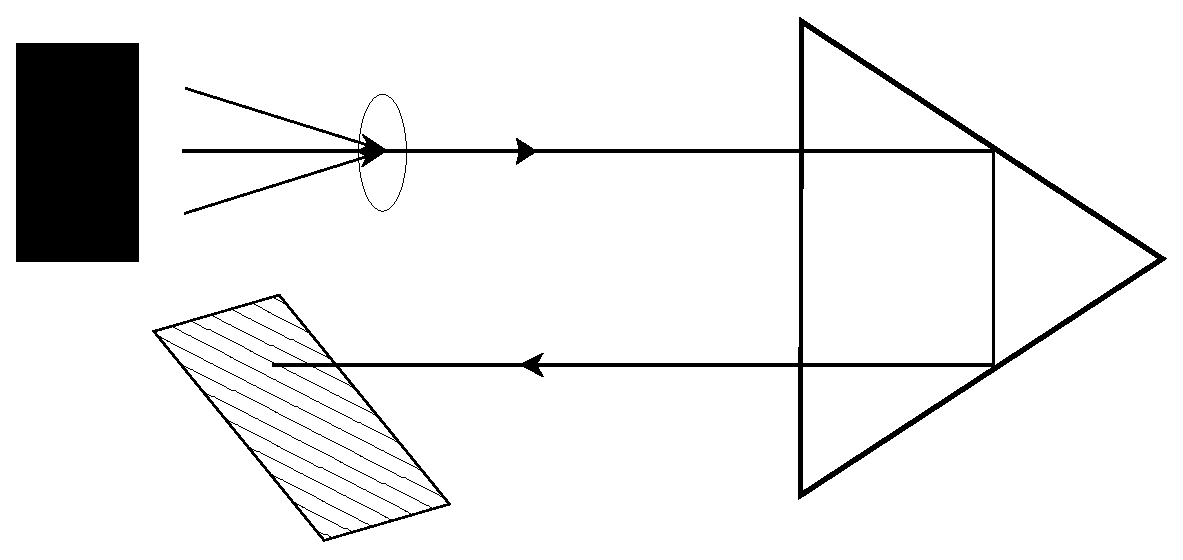
\includegraphics[height=5cm]{linediagram.eps}
%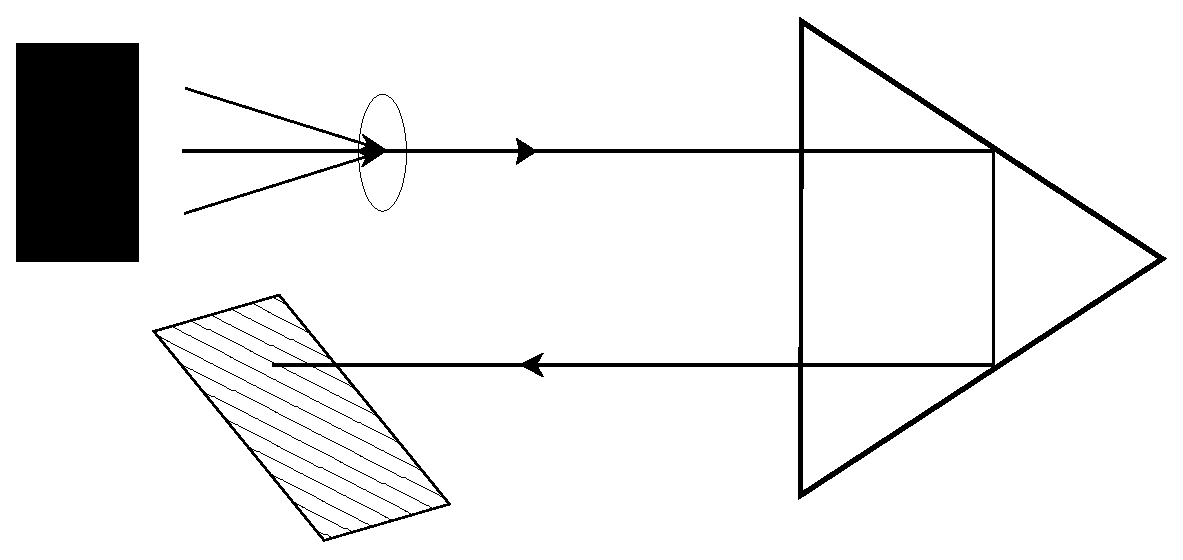
\includegraphics[height=5cm]{./linediagram.eps}
%\caption{This is an example of a numbered caption. \label{kuva1}}
%\end{figure}

% \begin{figure}[htb]
% \centering
% 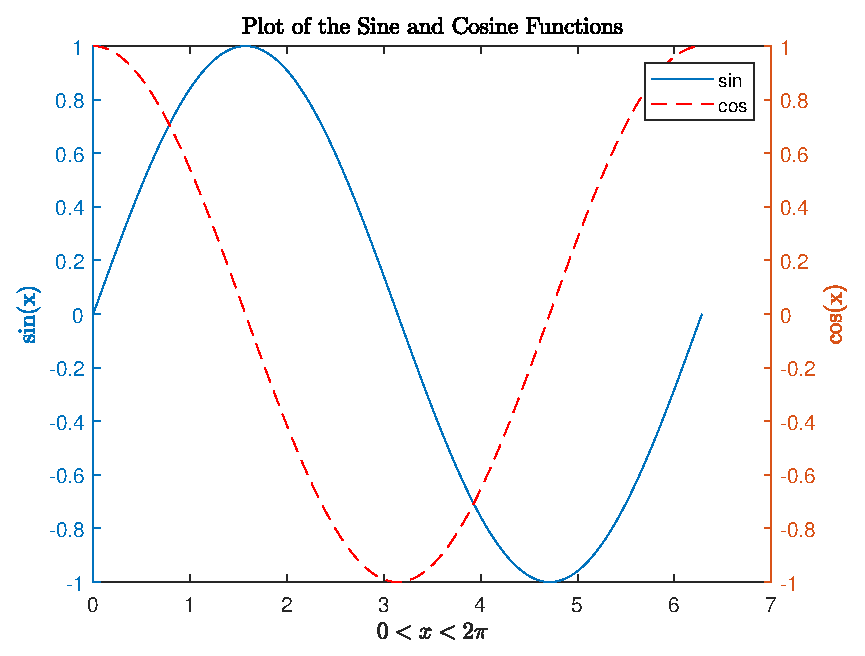
\includegraphics[height=5cm]{curves.eps}
% %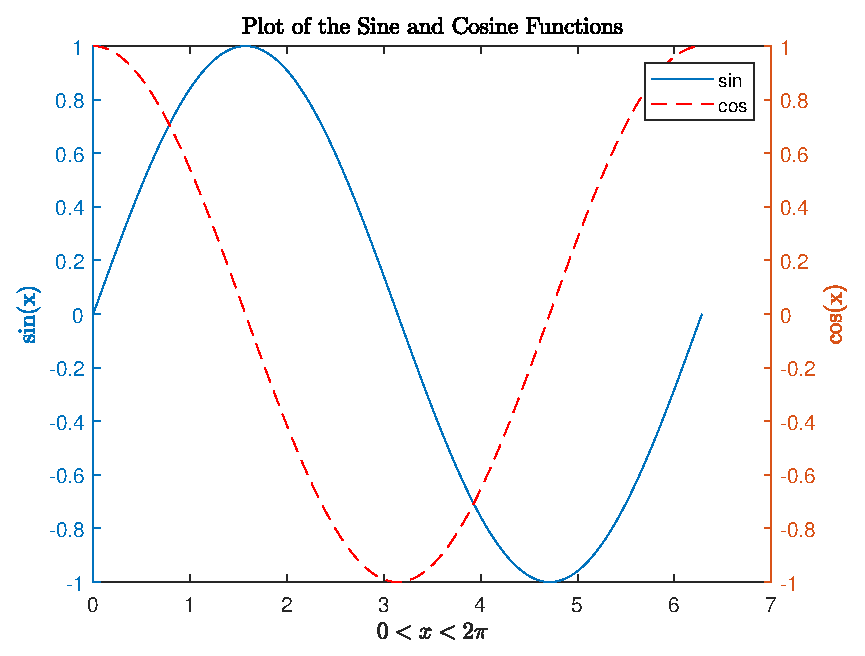
\includegraphics[height=5cm]{curves.eps}
% \caption{This is an example of a MATLAB graph. \label{kuva2}}
% \end{figure}


\clearpage
\section{Literature Review}


\clearpage
\section{\Acrlong{sispo}} \label{sec:sispo}

\gls{sispo} is a software package developed in python. It is separated in different sub-packages. The two main sub-packages are the \textit{sim} and the \textit{reconstruction} package. The third sub-package provides several image compression algorithms to test effects on reconstruction.

The software package is hosted on GitHub using a git version control system. Furthermore, the GitHub project management tools are used, including automated KanBan based projects, issue tracking and pull requests.

The most important python dependencies of \gls{sispo} are:
\begin{itemize}
    \item astropy: Astronomy package developed by \cite{robitaille2013astropy} and \cite{price2018astropy}
    \item Blender: 3D creation suite
    \item \textit{NumPy}: Scientific computing for python
    \item opencv: Computer vision library used for image processing
    \item OpenEXR: \gls{hdr} image reading and writing
    \item Orekit: Space dynamics library
\end{itemize}

It was attempted to reduce dependencies to other libraries as much as possible. Originally, both \textit{scikit-image} and \textit{opencv} were used. After a small benchmark between the two libraries, it was evident that \textit{opencv} performs three to seven times faster compared to \textit{scikit-image} (cf. \ref{sec:cvskimage}. Hence \textit{scikit-image} was completely replaced with equivalent \textit{opencv} functions. Additionally, it was attempted to use the \textit{opencv} package to replace the \textit{OpenEXR} dependency since it is not easy to install. However, this is currently not possible as the \textit{OpenEXR} implementation of \textit{opencv} does not provide an alpha channel and is generally less flexible.

To ease development, numerous parameters are silently assigned default values if not provided e.g. for an instrument. Therefore, all parameters should be explicitly set before running a simulation.

\gls{sispo} was developed in an attempt to logically separate the distinct steps involved of the entire processing pipeline. Such modularity eases further development as well as reduce unnecessary library imports to reduce memory consumption.

\subsection{User Interface}
The sispo package can be installed using pip and the GitHub project. If done, it will be installed into the site-packages folder of the used python environment. Additionally, an executable is installed, providing a \gls{cli} as user interface. The most recent possible input arguments are documented in the repository or by using the --help input. The most important arguments for the \gls{cli} are seen in Table \ref{tab:cli_args}.

\begin{table}[htpb]
\caption{Input arguments for sispo \gls{cli}}
\begin{tabular}{p{0.13\textwidth}|p{0.15\textwidth}|p{0.15\textwidth}|p{0.3\textwidth}}
\hline
\textbf{Name}                            & \textbf{Variable Name} & \textbf{Default Value}     & \textbf{Description}                                                                                                      \\ \hline
\multicolumn{1}{l|}{--help}              &                        & ---                        & Prints list of arguments with hints                                                                                       \\
\multicolumn{1}{l|}{-i}                  & i                      & data/input/definition.json & Path to a definition file that defines the settings                                                                 \\
\multicolumn{1}{l|}{-v}                  & v                      & False                      & Verbose output, logging information will also be displayed on STDOUT                                                      \\
\multicolumn{1}{l|}{--cli}               & cli                    & False                      & If the \gls{cli} flag is set, an interactive \gls{cli} will be started. NOT IMPLEMENTED. \\
\multicolumn{1}{l|}{--profile}           & profile                & False                      & If the profile flag is set, Python's cProfile will be used to profile \gls{sispo} execution              \\
\multicolumn{1}{l|}{--no-sim}            & with\_sim              & True                       & If flag is set, simulation step will be skipped                                                                           \\
\multicolumn{1}{l|}{--no-render}         & with\_render           & True                       & If flag is set, rendering step will be skipped                                                                            \\
\multicolumn{1}{l|}{--no-compression}    & with\_compression      & True                       & If flag is set, compression step will be skipped                                                                          \\
\multicolumn{1}{l|}{--no-reconstruction} & with\_reconstruction   & True                       & If flag is set, reconstruction step will be skipped                                                                       \\
\multicolumn{1}{l|}{--sim-only}          & sim\_only              & False                      & If flag is set, only simulation step will be done                                                                         \\
\multicolumn{1}{l|}{--sim-render-only}   & sim\_render\_only      & False                      & If flag is set, only simulation and rendering will be done                                                                \\
\multicolumn{1}{l|}{--render-only}       & render\_only           & False                      & If flag is set, only rendering will be done                                                                               \\
\multicolumn{1}{l|}{--compress-only}     & compress\_only         & False                      & If flag is set, only compression will be done                                                                             \\
\multicolumn{1}{l|}{--reconstruct-only}  & reconstruct\_only      & False                      & If flag is set, only reconstruction will be done                                                                         

\end{tabular}
\label{tab:cli_args}
\end{table}

The standard interface to be used is a \textit{definition.json} file which provides all input parameters in the \gls{json} format.

\gls{sispo} can be imported as a Python module. Execution is then started either by sispo.run() or sispo.main(), which are equivalent.

\subsection{Simulation Module}
The simulation module creates photo-realistic images by simulating a realistic trajectory of a \gls{sssb} and a spacecraft using Orekit. This trajectory and attitude data is then used to render four images per frame, one containing only the \gls{sssb}, one where the view is kept at a constant distance from the \gls{sssb}, one calibration reference image and one that renders a realistic star background using the \gls{ucac4}. Additionally, the date, the spacecraft position, \gls{sssb} position and their distance is stored as metadata. These images are composed to one image using photometry to calibrate the absolute light intensity of the different images in terms of realistic photon fluxes using the Johnson magnitude system \cite{bessel1979ubvri}. The composition process is explained in more detail in section \ref{sec:composition}

A run of the simulation package includes the following steps
\begin{enumerate}
    \item Propagate \label{enum:propagate}
    \item Render
\end{enumerate}

In the propagate step \ref{enum:propagate}, Orekit is used to determine state information of the \gls{sssb} and the spacecraft. The state information includes the date, position and the rotation angles of the \gls{sssb}. Propagation is defined by start and end date, number of steps, the timesampler mode and a slowmotion factor.
The timesampler mode determines whether the steps are distributed linear in time (mode 1, default) or whether an exponential model (mode 2) is used which takes more samples around the encounter. How many samples more are taken can be controlled with the slowmotion factor. Mode 2 is especially helpful when simulating a long period since far from the \gls{sssb} nucleus, there are only minor visible changes over longer periods.

The \textit{sim} sub-package was developed to contain all general information about the environment in the Environment class in order to have one consistent instance for constants. 

All images during the rendering and calibration process use the OpenEXR format to minimise the loss of information in intermediate steps.

The Orekit library runs a \gls{vm} to execute its Java code. Additionally, physical data is required which is currently distributed with the \textit{sim} sub-package. The \gls{vm} and physical data are initialised in the \textit{sim} main module and only afterwards other modules are imported which is why other modules do not include the Orekit initialisation. This approach was taken in order to reduce resource consumption by having several instances of the \gls{vm} running. Propagation is based on Orekit's KeplerianOrbit and KeplerianPropagator classes.

The initial state of the spacecraft is calculated based on the input parameters presented in \ref{tab:sc_enc_paras}. Only the three first parameters need to be given as input in the definition file.

\begin{table}[htb]
    \caption{Parameters that define the encounter state of the spacecraft.}
    \label{tab:sc_enc_paras}
    \begin{tabular}{p{0.23\textwidth}|p{0.06\textwidth}|p{0.62\textwidth}}
        Parameter           & Type  & Description                                                                                                                                                  \\ \hline
        encounter\_distance & float & Minimum distance between SSSB and spacecraft in meters                                                                                                       \\
        with\_terminator    & bool  & Determines whether the terminator is visible at the closest approach                                                                                         \\
        with\_sunnyside     & bool  & Determines whether the spacecraft passes the SSSB on the Sun facing side or the SSSB's side facing away from the Sun                                         \\
        sssb\_state         & tuple & \gls{sssb} state vector, including 3 position and 3 velocity components, at encounter. The spacecraft encounter state is calculated relative to this state vector. The \gls{sssb} state does not need to be set in the  definition file but is calculated based on the \gls{sssb} trajectory and encounter date.
    \end{tabular}
\end{table}

\subsubsection{Blender}
To render the \gls{sssb} and calibration images, Blender is used. A set of predefined settings is used for each scene while some parameters can be changed via the definition file. The rendering engine \textit{Cycles} is used to render photo-realistic, physics-based images from the Blender scenes.

Blender is interfaced using its Python bindings which need to be compiled manually (cf. \ref{sec:setup}. To control the behaviour of Blender the BlenderController class is used. It handles setting all defaults such as a black background and the creation of the default scene, SssbOnly. In addition, the BlenderController interfaces to the star catalogue and the compositor.

Since the images are composed and calibrated at a later step, described in \ref{sec:composition}, the settings shown in Table \ref{tab:color_space} are selected to not change the rendered raw images with Blender while saving.

\begin{table}[htpb]
\caption{Blender settings relevant to color space and are fixed to get raw images out of the Blender rendering process.}
\label{tab:color_space}
\begin{tabular}{p{0.25\textwidth}|p{0.08\textwidth}|p{0.57\textwidth}}
\textbf{Name}        & \textbf{Value} & \textbf{Description}                                                                                         \\ \hline
Color mode           & RGBA           & Use RGB and alpha channel.                                                                                   \\
Sequencer colorspace & Raw            & Color space sequencer uses linear color space.                                                               \\
View transform       & Raw            & No color space conversion.                                                                                   \\
Look                 & None           & No artistic effect is applied before color space conversion.                                                 \\
Film transparent     & True           & World background is transparent, i.e. alpha values can be used for image composition and proper occultation.
\end{tabular}
\end{table}

\begin{table}[htpb]
\caption{Blender settings that can be changed.}
\label{tab:blender_settings_input}
\begin{tabular}{p{0.12\textwidth}|p{0.1\textwidth}|p{0.7\textwidth}}
\textbf{Name}       & \textbf{Default Value} & \textbf{Description}                                                                                                         \\ \hline
Device     & AUTO          & Device used for rendering. "AUTO" attempts to use GPU, if not available uses CPU. \\
Samples    & 6             &                                                                                                                     \\
Exposure   & 0             & Exposure in stops, applied before display transform.                                                                \\
Resolution & ---           & Array determining number of pixels in x- and y-direction.                                                          
\end{tabular}
\end{table}

\subsubsection{Star Rendering} \label{sec:stars}
The background stars are rendered based on the star catalogue \gls{ucac4}. This catalogue includes stars up to magnitude 16. The \gls{fov} is determined based on the spacecraft camera in the SssbOnly scene. The edges of the \gls{fov} are calculated using the following equations

\begin{align}
    e_{right} = v_d + v_r \times \frac{s_w}{2 \times f}, \label{eq:edge_right} \\
    e_{left} = v_d - v_r \times \frac{s_w}{2 \times f}, \label{eq:edge_left} \\
    e_{upper} = v_d + v_u \times \frac{s_h}{2 \times f}, \label{eq:edge_upper} \\
    e_{lower} = v_d - v_u \times \frac{s_h}{2 \times f}, \label{eq:edge_lower}
\end{align}
where $e_{i}$ is a vector for the i-th edge of the \gls{fov}, $v_d$ is the direction vector of the camera, $v_r$ is the vector pointing right, $s_w$ is the camera sensor width, $s_h$ is the camera sensor height and $f$ is the focal length. These vectors are converted into their respective right ascension and declination using

\begin{align}
    \delta = \arcsin{(z)}, \label{eq:declination} \\
    \alpha = \arccos{\left(\frac{x}{\cos{\delta}}\right)} + \pi, \label{eq:right_ascension}
\end{align}
where $\delta$ is the declination and $\alpha$ the right ascension. The \gls{fov} is then defined as the right ascension and declination of the center point as well as the width and height. Using this information the star catalogue returns a list of visible stars with their right ascension and declination as well as their magnitude.

The star background is created by generating an image with twice the size of final image. The coordinates are converted from the right ascension and declination of each star into pixel coordinates. Afterwards setting the pixel value of each colour channel to the flux calculated from the magnitude. The resulting image is Gaussian filtered and downscaled to the final image size using local means. The alpha values of the entire image are set to one. Star background images are stored in the OpenEXR format. An example image is presented in Fig. \ref{fig:star_rendering}.

\begin{figure}[htpb]
    \centering
    
\includegraphics[width=\textwidth]{doc/thesis/0_figures/star_rendering/Stars_2017-08-15T115856-171000.png}
    \caption{Star background rendered using the method described in Section \ref{sec:stars}.}
    \label{fig:star_rendering}
\end{figure}


\subsubsection{Composition} \label{sec:composition}
Rendered images of Blender vary in absolute light intensity thus requiring calibration. For calibration, the Blender output is normalised by comparing the theoretical and real intensity of a calibration disk in the same conditions. This calibration is based on the Johnson magnitude system, also called the UBV photometric system \cite{bessel1979ubvri}. The V-band is used which is centered around \SI{550}{\nano\meter}.

The starting point for composition is a set of four images with the prefixes SssbOnly (cf. Fig. \ref{fig:comp_sssbonly}), SssbConstDist (cf. Fig. \ref{fig:comp_sssbconstdist}), LightRef (cf. Fig. \ref{fig:comp_lightref}) and Stars (cf. Fig. \ref{fig:comp_stars}). SssbOnly represents the view from the instrument. SssbConstDist is a follower camera at a constant distance of \SI{1000}{\kilo\meter} from the \gls{sssb}. LightRef is a defined reference model. Stars is an image of the star background. These images are then composed to a single final image. An example image set is shown in Fig. \ref{fig:comp_imageset}.

\begin{figure}[htb]
    \centering
    \begin{subfigure}[b]{0.47\textwidth}
        \centering
        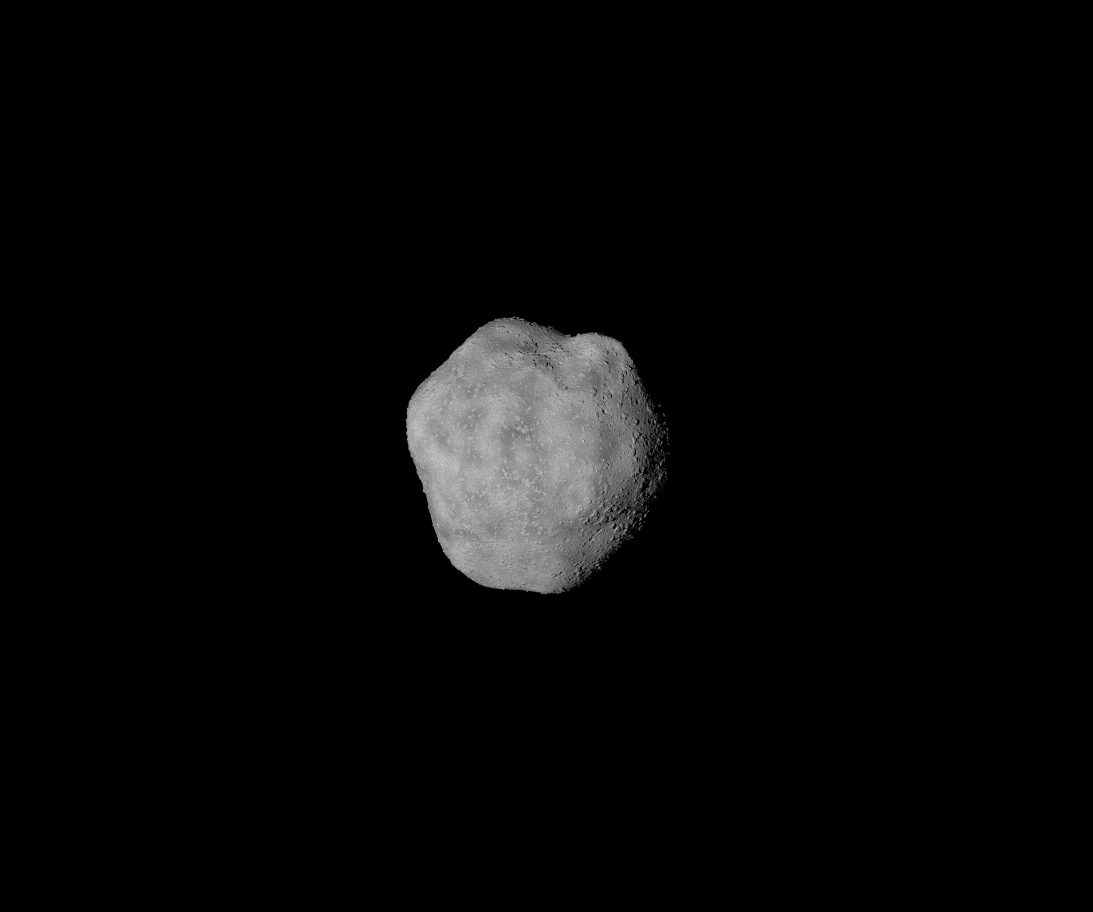
\includegraphics[width=\textwidth]{doc/thesis/0_figures/composition/SssbOnly_2017-08-15T115855-684000.png}
        \caption{SssbOnly}
        \label{fig:comp_sssbonly}
    \end{subfigure}
    \begin{subfigure}[b]{0.47\textwidth}
        \centering
        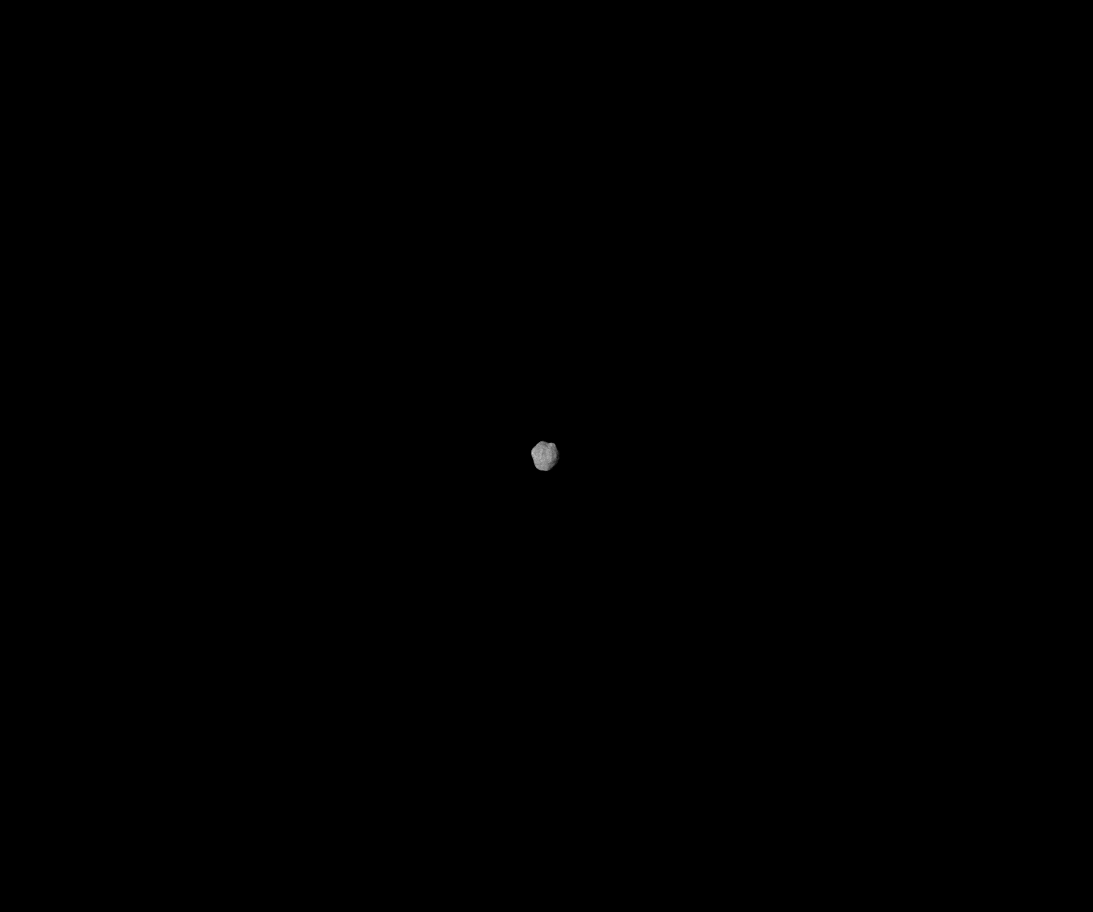
\includegraphics[width=\textwidth]{doc/thesis/0_figures/composition/SssbConstDist_2017-08-15T115855-684000.png}
        \caption{SssbConstDist}
        \label{fig:comp_sssbconstdist}
    \end{subfigure}
    \\
    \begin{subfigure}[b]{0.47\textwidth}
        \centering
        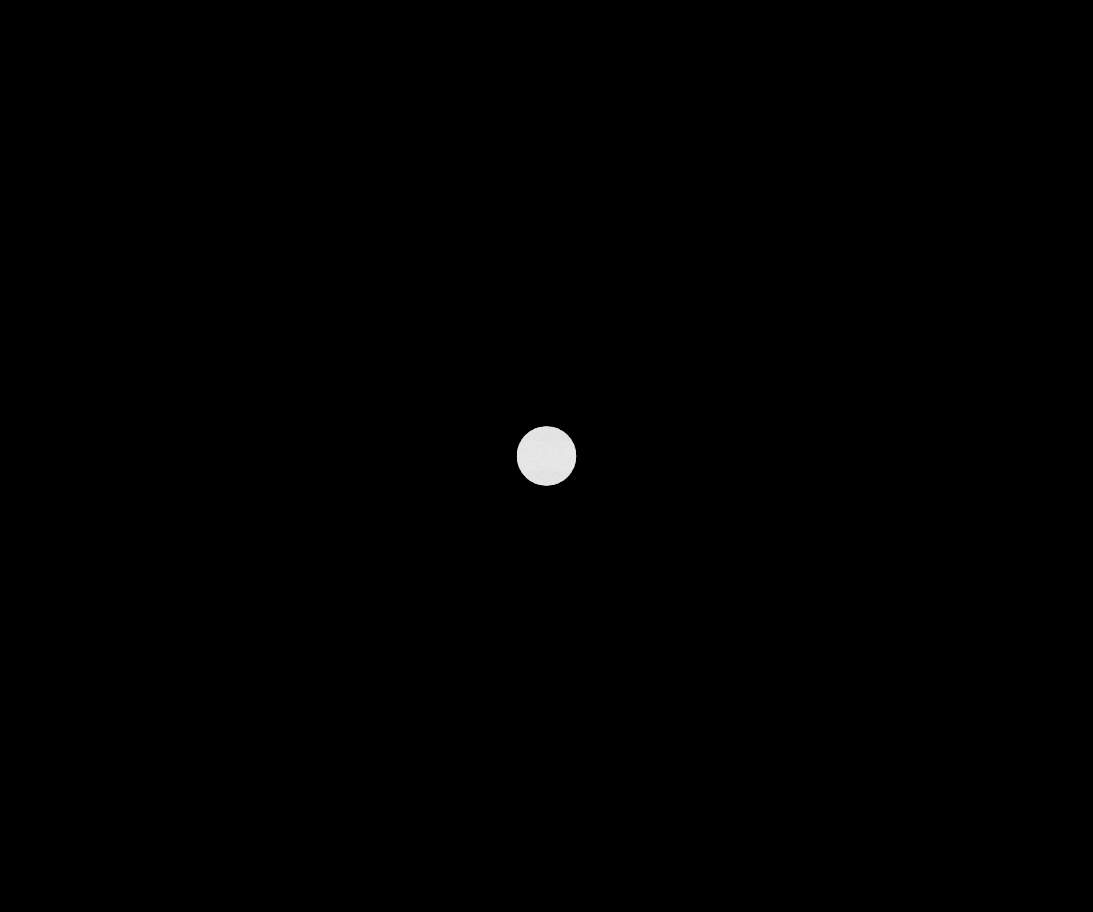
\includegraphics[width=\textwidth]{doc/thesis/0_figures/composition/LightRef_2017-08-15T115855-684000.png}
        \caption{LightRef}
        \label{fig:comp_lightref}
    \end{subfigure}
    \begin{subfigure}[b]{0.47\textwidth}
        \centering
        
\includegraphics[width=\textwidth]{doc/thesis/0_figures/composition/Stars_2017-08-15T115855-684000.png}
        \caption{Stars}
        \label{fig:comp_stars}
    \end{subfigure}
    \caption{Example set of images used for composition to the final rendering output.}
    \label{fig:comp_imageset}
\end{figure}

The reference used for photometric calibration is the solar photon flux in the V-band at \SI{1}{\astronomicalunit} calculated based on \cite{wirth}.

The photon flux is defined as,
\begin{align}
    F = F_0 \times \frac{d\lambda}{\lambda} \times 10^{-0.4 \times m}, \label{eq:comp_flux_0mag}
\end{align}
with $F_0$ being the flux at magnitude 0, $\frac{d\lambda}{\lambda}$ is a factor of 0.16 for the V-band, and $m$ is the object's magnitude. The V-band photon flux at $0~mag$ in SI units is \SI{5.4964e10}{\per\second \per\square\meter}. With a magnitude of $m_{\bigodot} = -26.74~mag$ at a distance of \SI{1}{\astronomicalunit}, the solar photon flux becomes \SI{4.36715206e+20}{\per\second\per\square\meter}.

In the first step, the reference photon flux per pixel is calculated using,
\begin{align}
        F_{ref} = F \times \left(\frac{\SI{1}{\astronomicalunit}}{d_{\bigodot}}\right)^2 \times \frac{A \times pix_A}{f^2 \times \pi}, \label{eq:comp_ref_flux}
\end{align}
where $F$ is the solar flux at \SI{1}{\astronomicalunit}, $d_{\bigodot}$ is the spacecraft distance from the Sun, $A$ is the aperture area, $pix_A$ is the area of a pixel and $f$ is the focal length.

For the star background, every pixel is calibrated according to Eq. \ref{eq:comp_cal_starmap}.
\begin{align}
        pix = pix_0 \times F_0 \times A \times \frac{F_{stars}}{S_{stars}}, \label{eq:comp_cal_starmap}
\end{align}
with $pix_0$ being the original pixel value, $F_0$ being the flux at magnitude 0, $A$ being the aperture area, $F_{stars}$ being the total flux of visible stars and $S_{stars}$ being the summed pixel value of one channel of a starmap.

Depending on the visible size of the \gls{sssb} in the image, either a point source \gls{sssb} image is generated and used or the \gls{sssb} image is calibrated. The point source is necessary if the \gls{sssb}'s nucleus is smaller than a pixel outputting wrong intensities.

The point source image is created by Gaussian filtering a single white pixel at the center of an image, oversized by a factor of five, and then downscaled to the original size using local means.

If the \gls{sssb} image is used, the reference intensity of the image is calculated as the mean of a \SI{70}{} square pixels of the light reference image.

Using the calibration factor defined as
\begin{align}
    f_c = \frac{F_{ref} \times I_{ref}}{\alpha}, \label{eq:comp_cal_fac}
\end{align}
where $F_{ref}$ is the reference flux, $I_{ref}$ is the reference intensity and $\alpha$ is the geometric albedo. Every pixel of the image is multiplied with this factor to produce the calibrated \gls{sssb} image. The star background and the calibrated \gls{sssb} image are merged taking the alpha channels into account. Using the alpha channel information provides proper occultation of the star background by the nucleus. For this, the \textit{film\_transparent} option of the Cycles rendering engine is activated.

The composed image is then multiplied by the quantum efficiency of the \gls{ccd}. This quantum efficiency currently includes all efficiencies to convert incoming photon flux into an electrical signal (pixel value). Afterwards, the image is Gaussian filtered and noise based on a Poisson distribution is added. The standard deviation for Gaussian filtering is calculated to approximate the diffraction pattern, defined as
\begin{align}
    \sigma = 0.45 \times \lambda \times \frac{f}{D}\times \frac{1}{pix_l} \times m, \label{eq:comp_sigma}
\end{align}
where $\sigma$ is the standard deviation, $\lambda$ is the instrument wavelength, $f$ is the focal length, $D$ is the aperture diameter, $pix_l$ is the length of one side of a pixel and $m$ is a multiplier for none diffraction limited systems (in our case $m = 2$. The noisy image is scaled to an interval $[0,1]$ by dividing through the maximum value. In case a point source \gls{sssb} is used, the maximum value is clipped to five times the maximum of the the reference if the maximum value of the merged image is above this threshold. The composed image using the data set shown in Fig. \ref{fig:comp_imageset} is presented Fig. \ref{fig:comp_composed}.

\begin{figure}
    \centering
    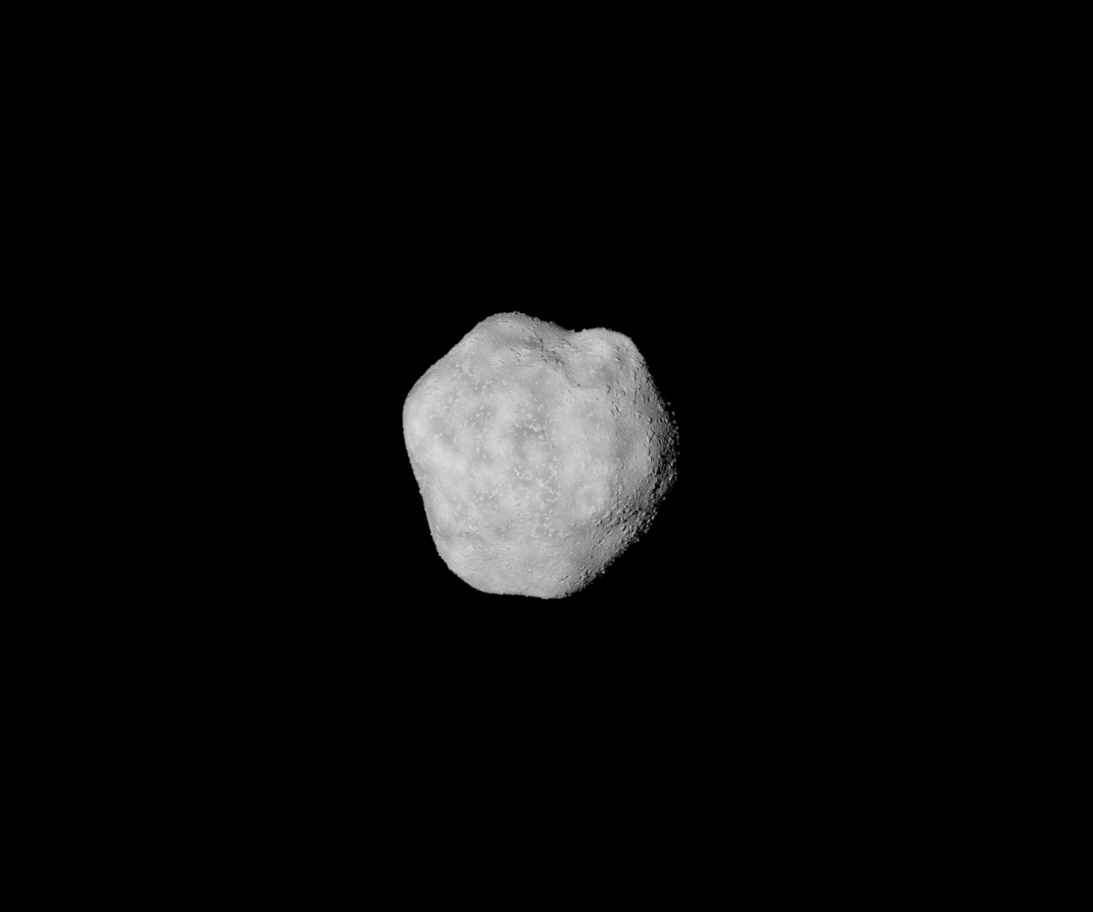
\includegraphics[width=\textwidth]{doc/thesis/0_figures/composition/Comp_2017-08-15T115854-575000.png}
    \caption{Composed image of the four images shown in Fig. \ref{fig:comp_imageset}}
    \label{fig:comp_composed}
\end{figure}

In a final step, the image values are scaled to the bit depth of the \gls{ccd}. The current maximum permissible bit depth is \SI{16}{bit} due to a substantial increase in code complexity for higher bit depths. This feature can be turned off by setting the \textit{with\_clipping} parameter to false.

An additional feature is to add an information box in the lower right corner of the image including the distance to the \gls{sssb} and the date. This feature can be turned off by setting the \textit{with\_infobox} parameter to false.

\subsection{Compression Module}
The compression module provides compression and decompression algorithms. These can be tested against different mission scenarios and image series to investigate the impact of compression and decompression on the scientific quality of the images. Table \ref{tab:compression_format} shows the available compression and decompression algorithms.

\begin{table}[htpb]
\caption{Lossless and lossy compression algorithms provided within \gls{sispo}.}
\label{tab:compression_format}
\begin{tabular}{l|l}
\textbf{Lossless Format} & \textbf{Lossy Formats} \\ \hline
png               & jpeg           \\
exr               & jpeg200        \\
bz2               & tiff           \\
gzip              &                \\
lzma              &                \\
zlib              &               
\end{tabular}
\end{table}

Independent of the algorithm, files are handled equally to. The images are loaded into \textit{NumPy} arrays inside Python to have a common raw format. Before encoding, the information is reduced to \SI{8}{\bit} since the reconstruction module only reads images with \SI{8}{\bit} colour depth correctly. Images are encoded with the respective algorithm and converted into a binary stream. A copy of this data is saved as a file in the raw folder. The raw binary data is then converted back to a \textit{NumPy} array and decoded to retrieve as much information as possible. Finally, the compressed and decompressed data is stored as a png file to not lose any further information.

The formats png, jpeg, jpeg2000 and tiff are implemented using \textit{OpenCV}. There are various settings for each format. A description can be found at \url{https://docs.opencv.org/4.1.2/d4/da8/group__imgcodecs.html#ga292d81be8d76901bff7988d18d2b42ac}.

The most important input parameter that is relevant to all algorithms is the "level" argument which describes either the compression level (from 1 to 9 for bz2, gzip, lzma, zlib and png, higher meaning more compression) or the quality level (from 1 to 10 for jpeg and jpeg2000, higher meaning better quality and less compression).

\subsection{Reconstruction Module}
The reconstruction module can be used to generate a 3D model of an object using a series of images. It provides a full Multi-View Stereo reconstruction data process pipeline. To achieve this, two libraries are used and combined and called using python. The first library is \gls{omvg} by \cite{openMVG}. The second library is \gls{omvs}. 
The common steps for the complete pipeline is comprised of the following steps:
\begin{enumerate}
    \item Read in images [ImageListing in \gls{omvg}]
    \item Compute visual features [ComputeFeatures in \gls{omvg}]
    \item Match computed features between different images [MatchFeatures in \gls{omvg}]
    \item Generate point cloud from matched features [IncrementalSfM in \gls{omvg}]
    \item Export to \gls{omvs} format [openMVG2openMVS in \gls{omvg}]
    \item Increase number of points in point cloud [DensifyPointCloud in \gls{omvs}]
    \item Create a mesh from the point cloud [ReconstructMesh in \gls{omvs}]
    \item Refine the generated mesh [RefineMesh in \gls{omvs}]
    \item Apply texture to mesh to create final 3D model [TextureMesh in \gls{omvs}]
\end{enumerate}

\subsection{Setup} \label{sec:setup}
\gls{sispo} can be setup with Linux and Windows. The default case used in this description is a Windows setup. Known differences or problems under Linux will be pointed out. While it should be possible to use a plain Python environment and pip, a miniconda environment manager was used for development. Also a C compiler is necessary. Linux provides the GCC, for Windows it is easiest to install Microsoft Visual Studio with \gls{msvc} and \gls{msbuild}. Another possibility when using Windows is to use vcpkg\footnote{Found at \url{https://github.com/microsoft/vcpkg}}. However, previously the openMVG and openMVS ports in vcpkg did not work. Vcpkg can also be used with Linux. However, there were unsolvable problems when using vcpkg so everything was installed natively.
For \gls{omvg}, \gls{omvs} and star\_cats it is necessary to have the executables in the correct folder for \gls{sispo} to function.\newline

\begin{figure}
    \dirtree{%
        .1 sispo.
            .2 build.
            .2 data.
                .3 input.
                .3 models.
                .3 sensor\_database.
                .3 UCAC4.
                    .4 u4b.
                    .4 u4i.
            .2 doc.
            .2 sispo.
                .3 compression.
                .3 reconstruction.
                .3 sim.
            .2 software.
                .3 blender.
                .3 miniconda.
                .3 openMVG.
                    .4 build\_openMVG.
                        .5 install.
                    .4 openMVG.
                .3 openMVS.
                    .4 build\_openMVS.
                        .5 install.
                    .4 openMVS.
                .3 star\_cats.
                    .4 build\_star\_cats.
                    .4 star\_cats.
                .3 vcpkg.
    }
    \caption{Directory structure after setup. No files are shown.}
    \label{fig:dir_tree}
\end{figure}
Figure \ref{fig:dir_tree} shows the assumed overall folder structure after installation. No sub-folders of the build folder or any files are shown.

To make \gls{sispo} perform well, it is beneficial to install the Nvidia CUDA Toolkit (https://developer.nvidia.com/cuda-downloads) in case an Nvidia graphics card is available.

In the following enumeration, commands intended to be run in a shell are highlighted with a grey box.

\begin{enumerate}
    \item Clone the GitHub repository onto the local machine \\ \shellcmd{git clone https://github.com/YgabrielsY/sispo.git}. The project provides a software folder which is intended to be used to install all following software.
    \item Setup (conda) environment with dependencies (to software/miniconda folder):
    \begin{enumerate}
        \item orekit 9.3.1, the current version 10.0 had issues when attempted to install. Also orekit needs a data package to function, it is distributed with \gls{sispo} in the sim module folder.
        \item astropy
        \item opencv
        \item OpenEXR\footnote{For Windows the pre-compiled package found at \url{https://www.lfd.uci.edu/~gohlke/pythonlibs/\#openexr} needs to be used because the pip or conda version do not work.}
        \item \textit{NumPy}
        \item Python\footnote{During development Python version 3.7 was used.}
    \end{enumerate}{}
    \item (Especially Windows) Install vcpkg to software/vcpkg folder, follow instructions at \url{https://github.com/microsoft/vcpkg}
    \item Install Blender as a python module (bpy)\footnote{During development Blender version 2.8 was used.}
    \begin{enumerate}
        \item Clone Blender git repository to software/blender/blender \\ \shellcmd{git clone git://git.blender.org/blender.git}
        \item Compile target bpy \shellcmd{make bpy}, this works also for Windows through the make.bat file provided with Blender
        \item When available: Activate CUDA in the cmake project and recompile
        \item Install bpy to python environment\footnote{Follow these instructions \url{https://blender.stackexchange.com/questions/117200/how-to-build-blender-as-a-python-module}}
    \end{enumerate}{}
    \item Install OpenMVG, follow instructions at \\ \url{https://github.com/openMVG/openMVG/blob/master/BUILD.md} or look for hints in the OpenMVG install script in the build folder.
    \begin{enumerate}
        \item Install dependencies according to instructions
        \item Clone OpenMVG GitHub repository to software/openMVG/openMVG \shellcmd{git clone --recursive https://github.com/openMVG/openMVG.git}
        \item Build to software/openMVG/build\_openMVG folder
        \item Install to software/openMVG/build\_openMVG/install folder
    \end{enumerate}
    \item Install OpenMVS, follow instructions at \\ \url{https://github.com/cdcseacave/openMVS/wiki/Building} or look at the OpenMVS install script in the build folder for hints.
    \begin{enumerate}
        \item Install dependencies according to instructions
        \item Clone OpenMVS GitHub repository to software/openMVS/openMVS \shellcmd{git clone https://github.com/cdcseacave/openMVS.git}
        \item Build to software/openMVS/build\_openMVS folder
        \item Install to software/openMVS/build\_openMVS/install folder
    \end{enumerate}
    \item Install star\_cats
    \begin{enumerate}
        \item Clone star\_cats GitHub repository to software/star\_cats/star\_cats \\ \shellcmd{git clone https://github.com/Bill-Gray/star\_cats.git}
        \item Build to software/star\_cats/build\_star\_cats \shellcmd{make}
    \end{enumerate}
    \item Download UCAC4 star catalog to data/UCAC4, use either:
    \begin{enumerate}
        \item the build/data/download\_ucac4.sh script
        \item download the folder u4b and u4i directly from \\ \url{http://casdc.china-vo.org/mirror/UCAC/UCAC4/}
    \end{enumerate}
\end{enumerate}{}

\subsection{Performance}
\subsubsection{Image processing benchmark} \label{sec:cvskimage}
The original codebase used the \gls{skimage} and OpenCV libraries. In order to reduce the number of dependencies, the relevant functions of the two libraries were benchmarked. For this comparison, OpenCV functions were used to create the same behaviour as the respective \gls{skimage} function. The benchmark compares the performance of the Gaussian filter and a special case of image resizing using local means. A set of five images is selected and are shown in Appendix \ref{sec:app_cvskimage}. Two star images were selected due to the large variance in the number of visible stars. The selected images represent extreme cases with 1804 (Stars1) and 51338 stars (Stars2).

Two computers are used for the benchmark. A laptop with \SI{8}{\giga\byte} \gls{ram}, an Intel i7-6700HQ with 4 cores at \SI{2.6}{\giga\hertz} and Windows 10. The second is a workstation computer with \SI{16}{\giga\byte} of \gls{ram}, an Intel i7-8700 with 6 cores at \SI{3.2}{\giga\hertz} and Ubuntu 18.04.3 LTS.

To compare the performance between the two libraries the ratio of execution time is used. The ratio is defined as
\begin{align}
    Ratio = \frac{t_{skimage}}{t_{opencv}}, \label{eq:bm_exec_ratio}
\end{align}
where $t_{skimage}$ is the execution time of \gls{skimage} and $t_{opencv}$ is the execution time of OpenCV. Each command is executed and timed for 1000 times. The lowest value is chosen as the result, since higher values are rather influenced by other processes running on the respective machine than the relevant code snippet itself \cite{timeit2020}.

Figure \ref{fig:bm_comparison} shows the execution time ratios with their averages over set of images. A ratio larger than one corresponds to a longer execution time of \gls{skimage}. OpenCV outperforms \gls{skimage} for both tests on both computers. The maximum absolute difference between pixel values of images is \SI{1.486e-6}{} and \SI{7.153e-7}{} for the Gaussian filtered and the resized images respectively. Such differences are irrelevant considering \gls{ccd} sensor color depths of \SI{16}{bit}.

%Maximum error gauss:  1.4864218655930017e-06
%Maximum error resize:  7.152557373046875e-07

\begin{figure}[htb]
    \centering
    \begin{subfigure}[b]{0.47\textwidth}
        \centering
        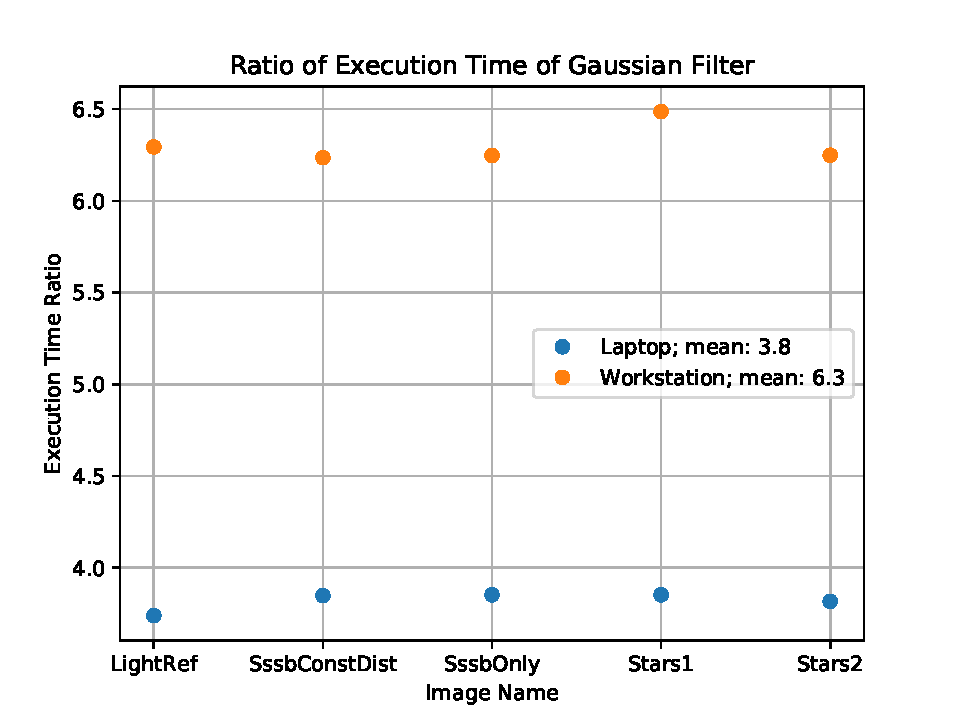
\includegraphics[width=\textwidth]{doc/thesis/0_figures/cv_skimage/Comparison_Gaussian}
        \caption{Gaussian filtering.}
        \label{fig:bm_comparison_gauss}
    \end{subfigure}
    \begin{subfigure}[b]{0.47\textwidth}
        \centering
        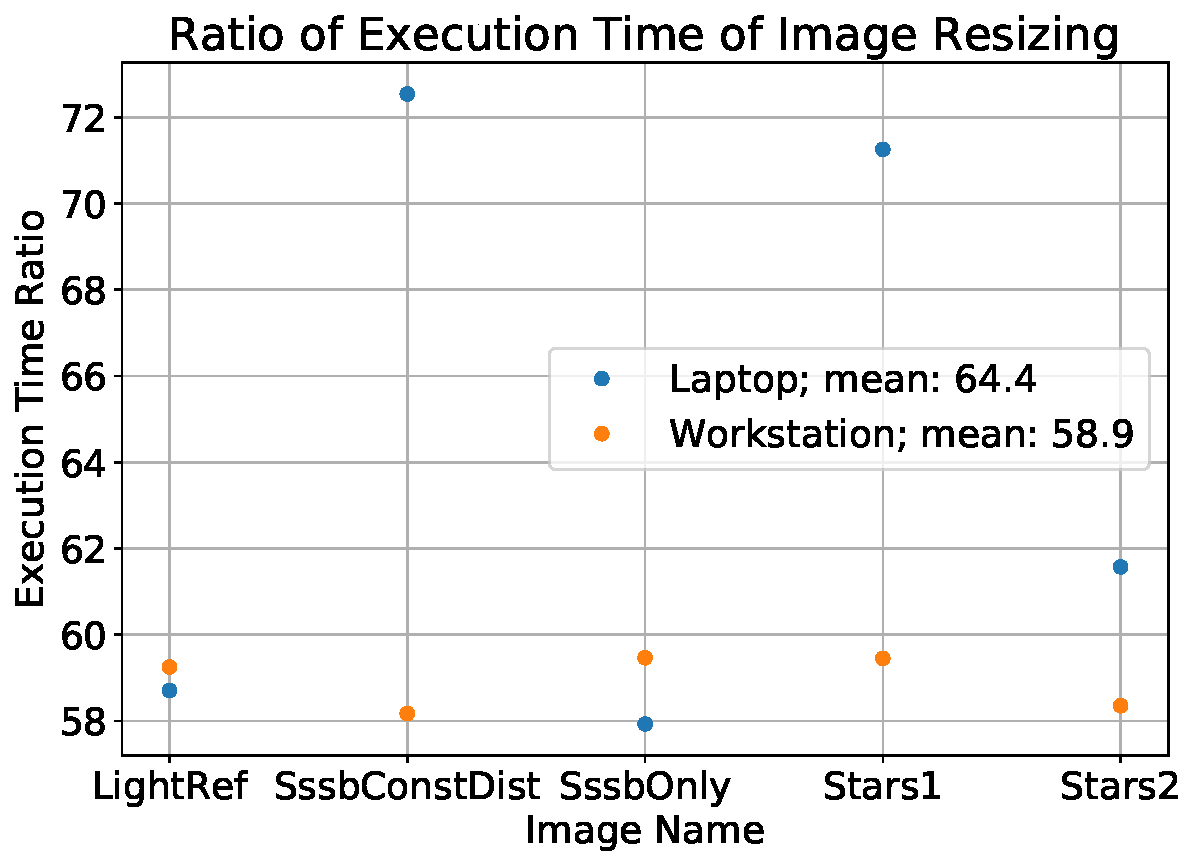
\includegraphics[width=\textwidth]{doc/thesis/0_figures/cv_skimage/Comparison_Resize}
        \caption{Resizing.}
        \label{fig:bm_comparison_res}
    \end{subfigure}
    \caption{Comparison of execution time ratios of Gaussian filtering and resizing five images using OpenCV and \gls{skimage} on two computers. Values $> 1$ correspond to OpenCV being faster. The mean values are given in the legend.}
    \label{fig:bm_comparison}
\end{figure}

For our case, OpenCV has a clear performance advantage over the \gls{skimage} library, hence only OpenCV is being used. In addition to the performance advantages, OpenCV might also be used to replace the OpenEXR dependency in the future, if OpenCV's OpenEXR implementation includes alpha channel support\footnote{A GitHub issue was created at \url{https://github.com/YgabrielsY/sispo/issues/128} that links to the relevant OpenCV GitHub issue.}.

\subsection{Future Developments}
There are several issues left open within the \gls{sispo} software package. First, there is currently no realistic model of spacecraft attitude motion and control implemented. The camera of the simulation environment is perfectly oriented towards the centre of the \gls{sssb}'s nucleus during the entire simulation. Realistic rotation should cover at least two effects, motion blur due to instantaneous rotation velocities of spacecraft and off-centre pointing due to control inaccuracies. Furthermore, it is necessary to include  image distortions such as astigmatism, bokeh, coma, field curvature, glare. Moreover, it is necessary to include a gas and dust environment around the nucleus. From a technical perspective, a proper simulation of the data transmission should be included. For example, a realistic simulation for packet loss. The ultimate goal is to develop a prioritisation algorithm for the images which should prioritise data transmission on packet level.
Moreover, multi-instumrent capability was intended as well as including multiple \gls{sssb}s in the future to allow more complex simulations including e.g. a binary system.
Furthermore, the shader used to create the \gls{sssb} models should be developed further. The interface for it should be included into \gls{sispo} and restricted to values that create reasonable shaped outputs.
An attempt to include a HAPKE model via the synthspace package \url{https://github.com/oknuutti/synthspace} was unsuccessful. However, it would be interesting to compare the results of Blender and the HAPKE model. A HAPKE model is substantially faster while providing less detail though possibly still sufficient for some cases.

THOUGHTS:\\
-default data set, different compression and reconstruction\\
    -compressions: png, jpg2000 quality 1000, jpg2000 quality 500, jpg2000 quality 100, jpg2000 quality 10\\
-different trajectories: default : 400 km, 100km, 1000km\\
-different lighting situations\\
-different models 100m, 1km, 10km


\clearpage

\section{Results} \label{sec:results}

\begin{table}[htpb]
\caption{Simulation parameters}
\label{tab:sim_params}
\begin{tabular}{l|lll}
ID      & \gls{sssb} Size \SI{}{\kilo\meter} & Encounter Distance \SI{}{\kilo\meter} & Compression Method      \\
Default & 1                                                                                                        & 400                                                                                          & png                     \\
1       & 1                                                                                                        & 400                                                                                          & jpeg2000: quality 1000  \\
2       & 1                                                                                                        & 400                                                                                          & jpeg2000: quality 100   \\
3       & 1                                                                                                        & 400                                                                                          & jpeg2000: quality 10    \\
4       & 1                                                                                                        & 100                                                                                          & png                     \\
5       & 1                                                                                                        & 100                                                                                          & jpeg2000 : quality 1000 \\
6       & 1                                                                                                        & 100                                                                                          & jpeg2000: quality 100   \\
7       & 1                                                                                                        & 100                                                                                          & jpeg200: quality 10     \\
8       & 1                                                                                                        & 1000                                                                                         & png                     \\
9       & 1                                                                                                        & 1000                                                                                         & jpeg2000 : quality 1000 \\
10      & 1                                                                                                        & 1000                                                                                         & jpeg2000 : quality 100  \\
11      & 1                                                                                                        & 1000                                                                                         & jpeg2000 : quality 10   \\
12      & 10                                                                                                       & 400                                                                                          & png                     \\
13      & 10                                                                                                       & 400                                                                                          & jpeg2000 : quality 1000 \\
14      & 10                                                                                                       & 400                                                                                          & jpeg2000 : quality 100  \\
15      & 10                                                                                                       & 400                                                                                          & jpeg2000 : quality 10   \\
16      & 0.1                                                                                                      & 400                                                                                          & png                     \\
17      & 0.1                                                                                                      & 400                                                                                          & jpeg2000 : quality 1000 \\
18      & 0.1                                                                                                      & 400                                                                                          & jpeg2000 : quality 100  \\
19      & 0.1                                                                                                      & 400                                                                                          & jpeg2000 : quality 10  
\end{tabular}
\end{table}
%\section{Tulokset}



\clearpage

\section{Conclusion} \label{sec:conclusion}
\subsection{Summary}
A first implementation for simulating a \gls{sssb} flyby mission could be created. It is capable of rendering images, compressing and decompressing these images and reconstructing a textured \gls{3d} model.
The rendering output of \gls{sispo} better resembles asteroids than comets.

It was possible to show the influence of compression on images. However, quantifying image quality solely on the number of reconstructed points

\subsection{Future Developments}
There are several issues left open within the \gls{sispo} software package. First, there is currently no realistic model of spacecraft attitude motion and control implemented. The camera of the simulation environment is perfectly oriented towards the centre of the \gls{sssb}'s nucleus during the entire simulation. Realistic rotation should cover at least two effects, motion blur due to instantaneous rotation velocities of spacecraft and off-centre pointing due to control inaccuracies. Furthermore, it is necessary to include  image distortions such as astigmatism, bokeh, coma, field curvature, glare.

Currently, \gls{sispo} assumes that an instrument always has \gls{rgb} channels. Since many \gls{ccd}s used in deep space are only \gls{bw} cameras, a possibility to choose either \gls{rgb} or \gls{bw} should be implemented.

Moreover, it is necessary to include a gas and dust environment around the nucleus. From a technical perspective, a proper simulation of the data transmission should be included. For example, a realistic simulation for packet loss. The ultimate goal is to develop a prioritisation algorithm for the images which should prioritise data transmission on packet level.
Moreover, multi-instrument capability was intended as well as including multiple \gls{sssb}s in the future to allow more complex simulations including e.g. a binary system.

Furthermore, the shader used to create the \gls{sssb} models should be developed further. The interface for it should be included into \gls{sispo} and restricted to values that create reasonable shaped outputs. Additionally, the shader should also represent comet surfaces better. Furthermore, since most of the execution time is spent rendering, the shader should be developed to be less computationally heavy.

An attempt to include a HAPKE model via the synthspace package \url{https://github.com/oknuutti/synthspace} was unsuccessful. However, it would be interesting to compare the results of Blender and the HAPKE model. A HAPKE model is substantially faster while being less accurate though possibly still sufficient for some cases.

To improve computational performance and make image compression and possible data transmission more realistic, image cropping should be added. A substantial part of an image far from a nucleus is black which could be cropped away to reduce the amount of data for the computation and the system itself.
%\section{Yhteenveto}


\clearpage
%% L\"ahdeluettelo

\thesisbibliography
\printbibliography
%\bibliographystyle{plain}
%\begin{thebibliography}{99}
%\bibliographystyle{ieeetr}
%\bibliography{99_references}
%\end{thebibliography}

%% Appendices
%% If you don't have appendices, remove \clearpage and \thesisappendix below.
\clearpage

\thesisappendix

\section{Esimerkki liitteest\"a\label{LiiteA}}

\section{Esimerkki liitteest\"a\label{LiiteA}}
Liitteet eiv\"at ole opinn\"aytteen kannalta v\"altt\"am\"att\"omi\"a ja 
opinn\"aytteen tekij\"an on 
kirjoittamaan ryhtyess\"a\"an hyv\"a ajatella p\"arj\"a\"av\"ans\"a ilman liitteit\"a.
Kokemattomat kirjoittajat, jotka ovat huolissaan
tekstiosan pituudesta, paisuttavat turhan 
helposti liitteit\"a pit\"a\"akseen tekstiosan pituuden annetuissa rajoissa.
T\"all\"a tavalla ei synny hyv\"a\"a opinn\"aytett\"a.   

Liite on itsen\"ainen kokonaisuus, vaikka se t\"aydent\"a\"akin tekstiosaa.
Liite ei siten ole pelkk\"a listaus, kuva tai taulukko, vaan 
liitteess\"a selitet\"a\"an aina sis\"all\"on laatu ja tarkoitus. 

Liitteeseen voi laittaa esimerkiksi listauksia. Alla on 
listausesimerkki t\"am\"an liitteen luomisesta. 

%% Verbatim-ymp\"arist\"o ei muotoile tai tavuta teksti\"a. Fontti on monospace.
%% Verbatim-ymp\"arist\"on sis\"all\"a annettuja komentoja ei LaTeX k\"asittele. 
%% Vasta \end{verbatim}-komennon j\"alkeen jatketaan k\"asittely\"a.
\begin{verbatim}
	\clearpage
	\appendix
	\addcontentsline{toc}{section}{Liite A}
	\section*{Liite A}
	...
	\thispagestyle{empty}
	...
	teksti\"a
	...
	\clearpage
\end{verbatim}

Kaavojen numerointi muodostaa liitteiss\"a oman kokonaisuutensa:
\begin{align}
d \wedge A &= F, \label{liitekaava1}\\
d \wedge F &= 0. \label{liitekaava2}
\end{align}


\clearpage
\section{Toinen esimerkki liitteest\"a\label{LiiteB}}

\section{Shader Node Network} \label{sec:shader_node}

\begin{figure}[htb]
    \centering
    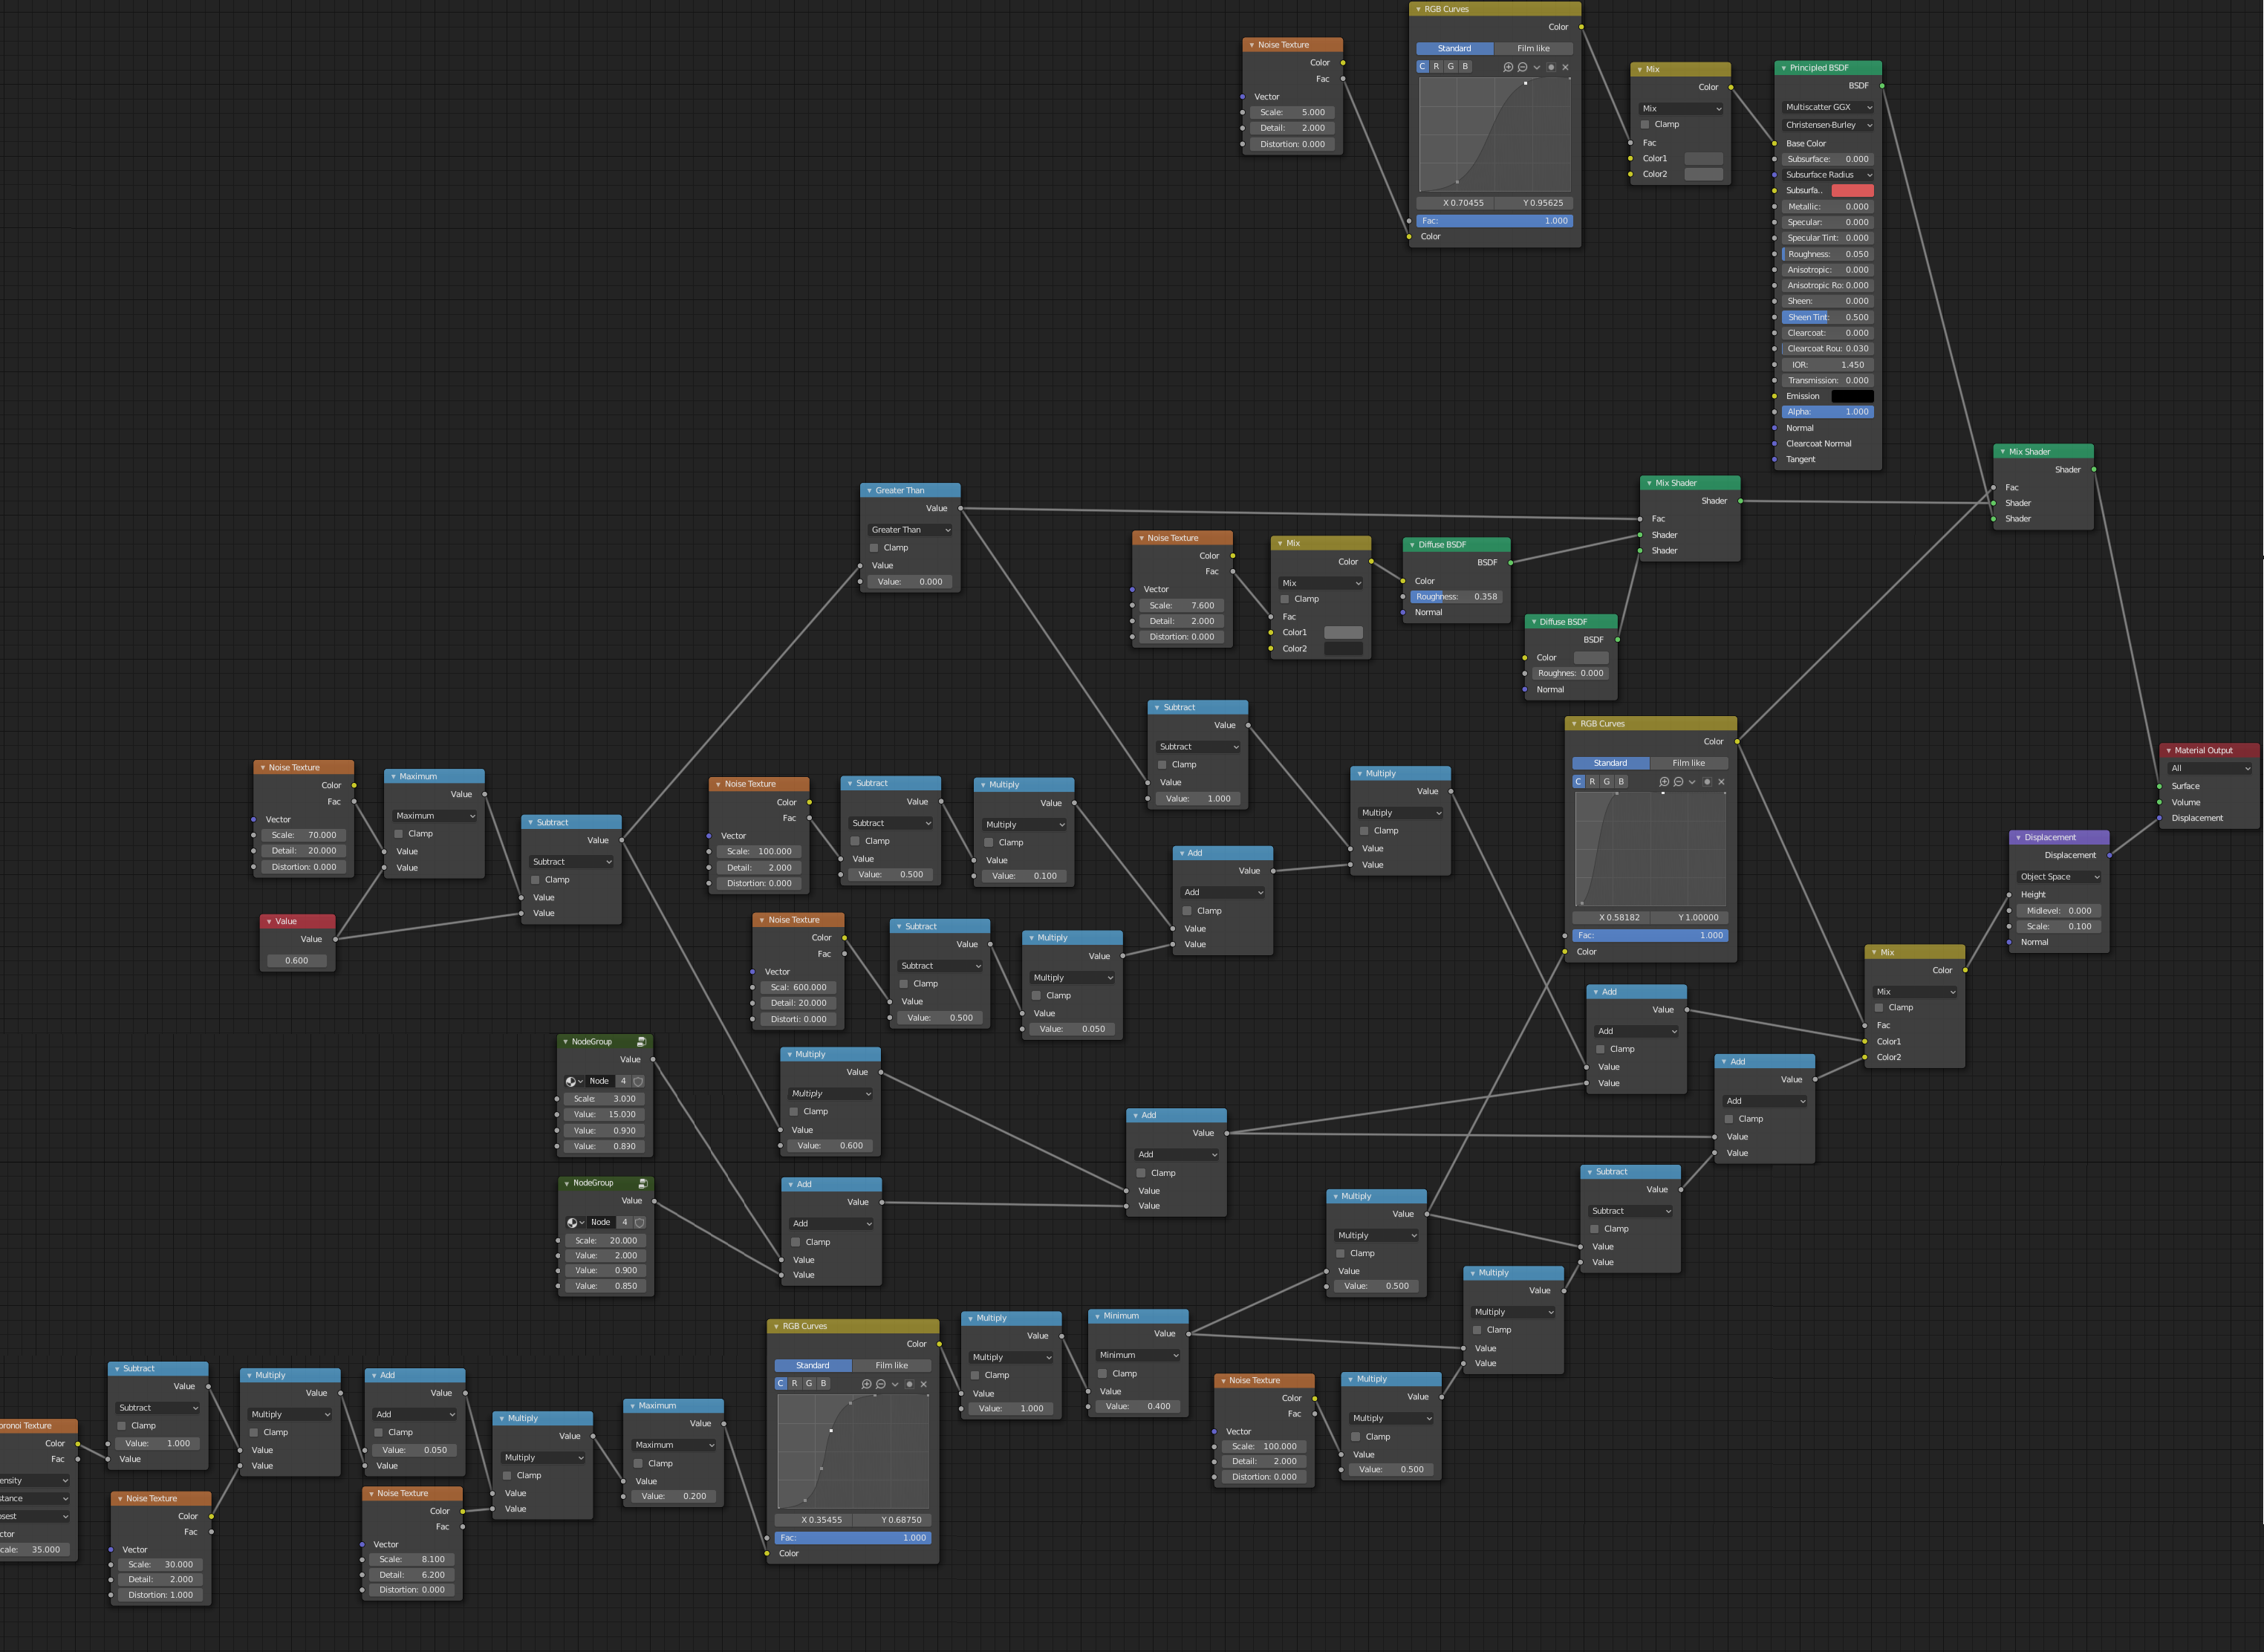
\includegraphics[height=.97\textwidth, angle=90]{doc/thesis/0_figures/procedural_terrain/node_network_highres.png}
    \caption{High resolution image of the shader node network used in \gls{sispo}.}
    \label{fig:node_highres}
\end{figure}


%\section{Toinen esimerkki liitteest\"a\label{LiiteB}}
%% Liitteiden kaavat, taulukot ja kuvat numeroidaan omana kokonaisuutenaan
%%
%% Equations, tables and figures have their own numbering in Appendices
%\renewcommand{\theequation}{B\arabic{equation}}
%\setcounter{equation}{0}  
%\renewcommand{\thefigure}{B\arabic{figure}}
%\setcounter{figure}{0}
%\renewcommand{\thetable}{B\arabic{table}}
%\setcounter{table}{0}

% Liitteiss\"a voi my\"os olla kuvia, jotka
% eiv\"at sovi leip\"atekstin joukkoon:
% %% Ymp\"arist\"on figure parametrit htb pakottavat
% %% kuvan t\"ah\"an, eik\"a LaTeX yrit\"a siirrell\"a niit\"a
% %% hyv\"aksi katsomaansa paikkaan. 
% %% Ymp\"arist\"o\"a center voi k\"aytt\"a\"a \centering-
% %% komennon sijaan
% %%
% %% Example of a figure, note the use of htb parameters which force
% %% the figure to be inserted here
% \begin{figure}[htb]
% \begin{center}
% 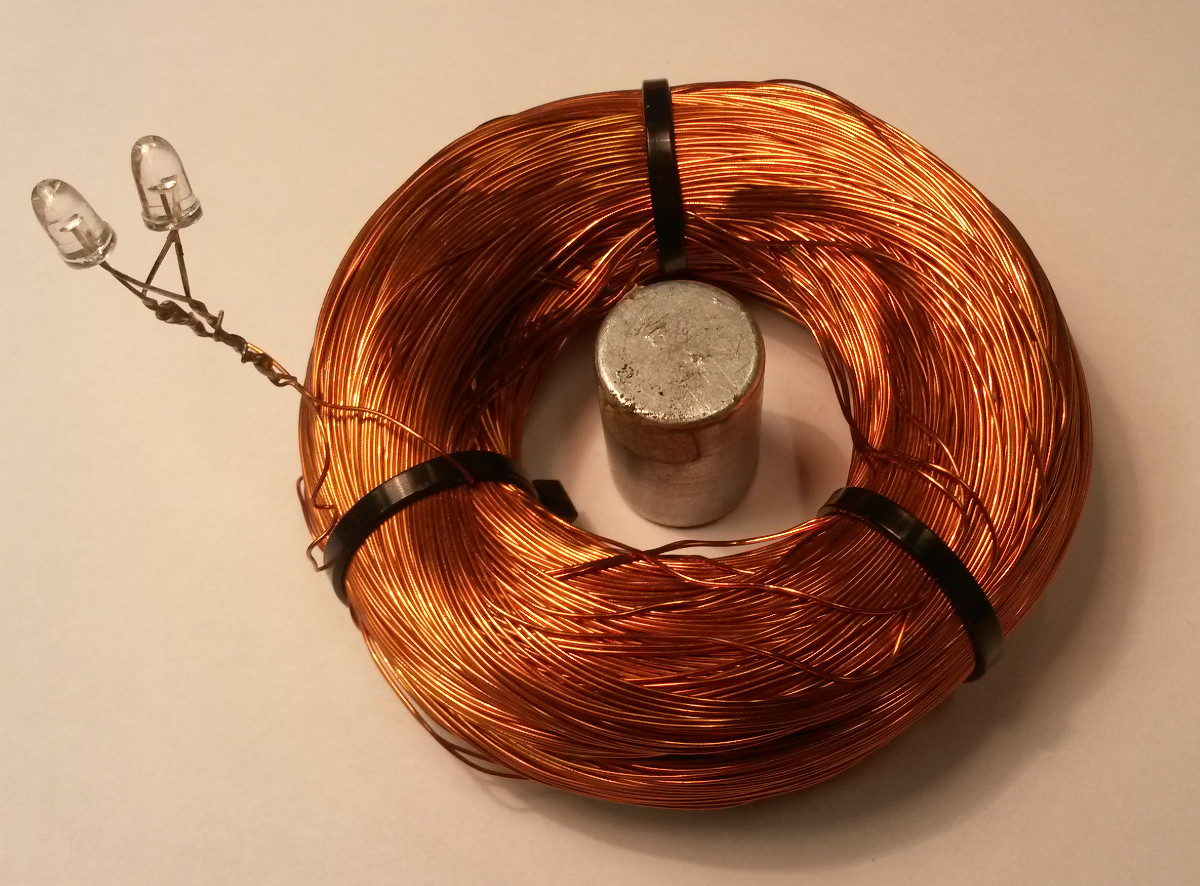
\includegraphics[height=8cm]{doc/thesis/0_figures/ledspole.jpg}
% \end{center}
% \caption{Kuvateksti, jossa on liitteen numerointi}
% \label{liitekuva}
% \end{figure}
% %%
% Liitteiden taulukoiden numerointi on kuvien ja kaavojen kaltainen:
% \begin{table}[htb]
% \caption{Taulukon kuvateksti.}
% \label{liitetaulukko}
% \begin{center}
% \fbox{
% \begin{tabular}{lp{0.5\linewidth}}
% 9.00--9.55  & K\"aytett\"avyystestauksen tiedotustilaisuus (osanottajat
% ovat saaneet s\"ahk\"opostitse valmistautumisteht\"av\"at, joten tiedotustilaisuus
% voidaan pit\"a\"a lyhyen\"a).\\
% 9.55--10.00 & Testausalueelle siirtyminen
% \end{tabular}}
% \end{center}
% \end{table}
% Kaavojen numerointi muodostaa liitteiss\"a oman kokonaisuutensa:
% \begin{align}
% T_{ik} &= -p g_{ik} + w u_i u_k + \tau_{ik},  \label{liitekaava3} \\
% n_i    &= n u_i + v_i.                      \label{liitekaava4}
% \end{align}

\clearpage
\section{Image Set for Image Processing Benchmark} \label{sec:app_cvskimage}


\begin{figure}[htb]
    \begin{center}
        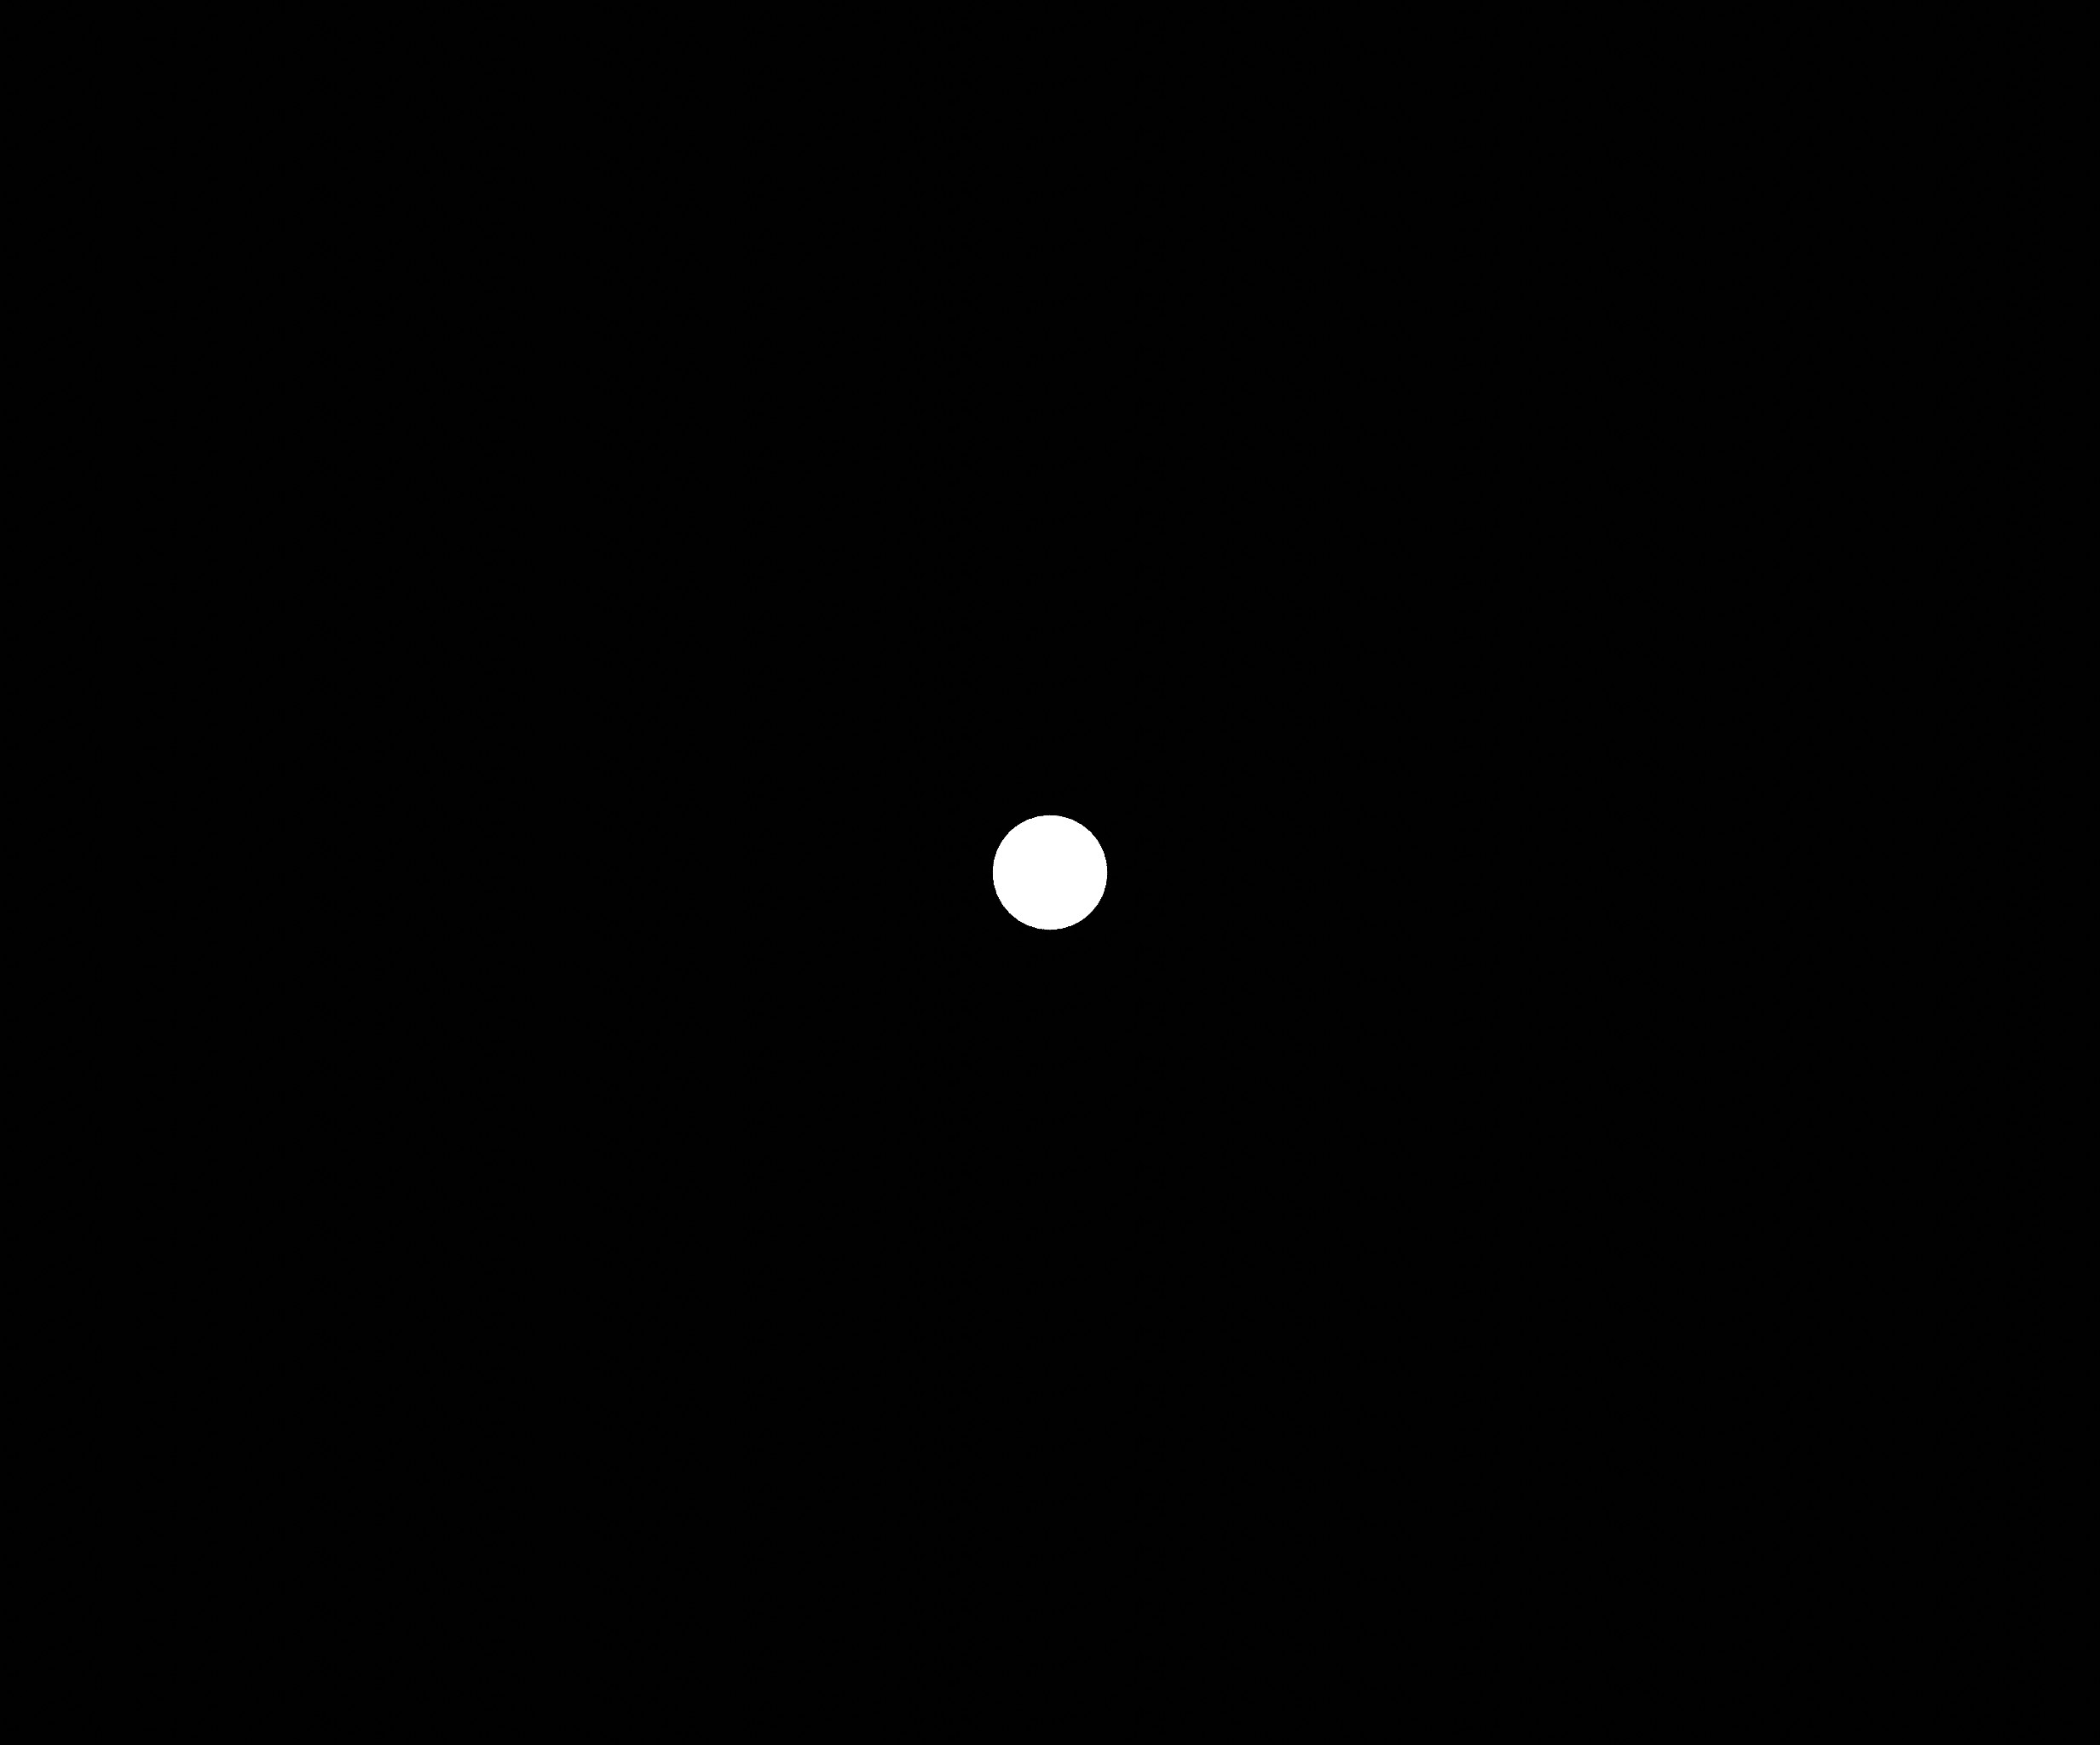
\includegraphics[height=8cm]{doc/thesis/0_figures/cv_skimage/LightRef_2017-08-15T115851-679000.jpg}
    \end{center}
    \caption{LightRef image used in benchmark.}
    \label{fig:bm_light_ref}
\end{figure}

\begin{figure}[htb]
    \begin{center}
        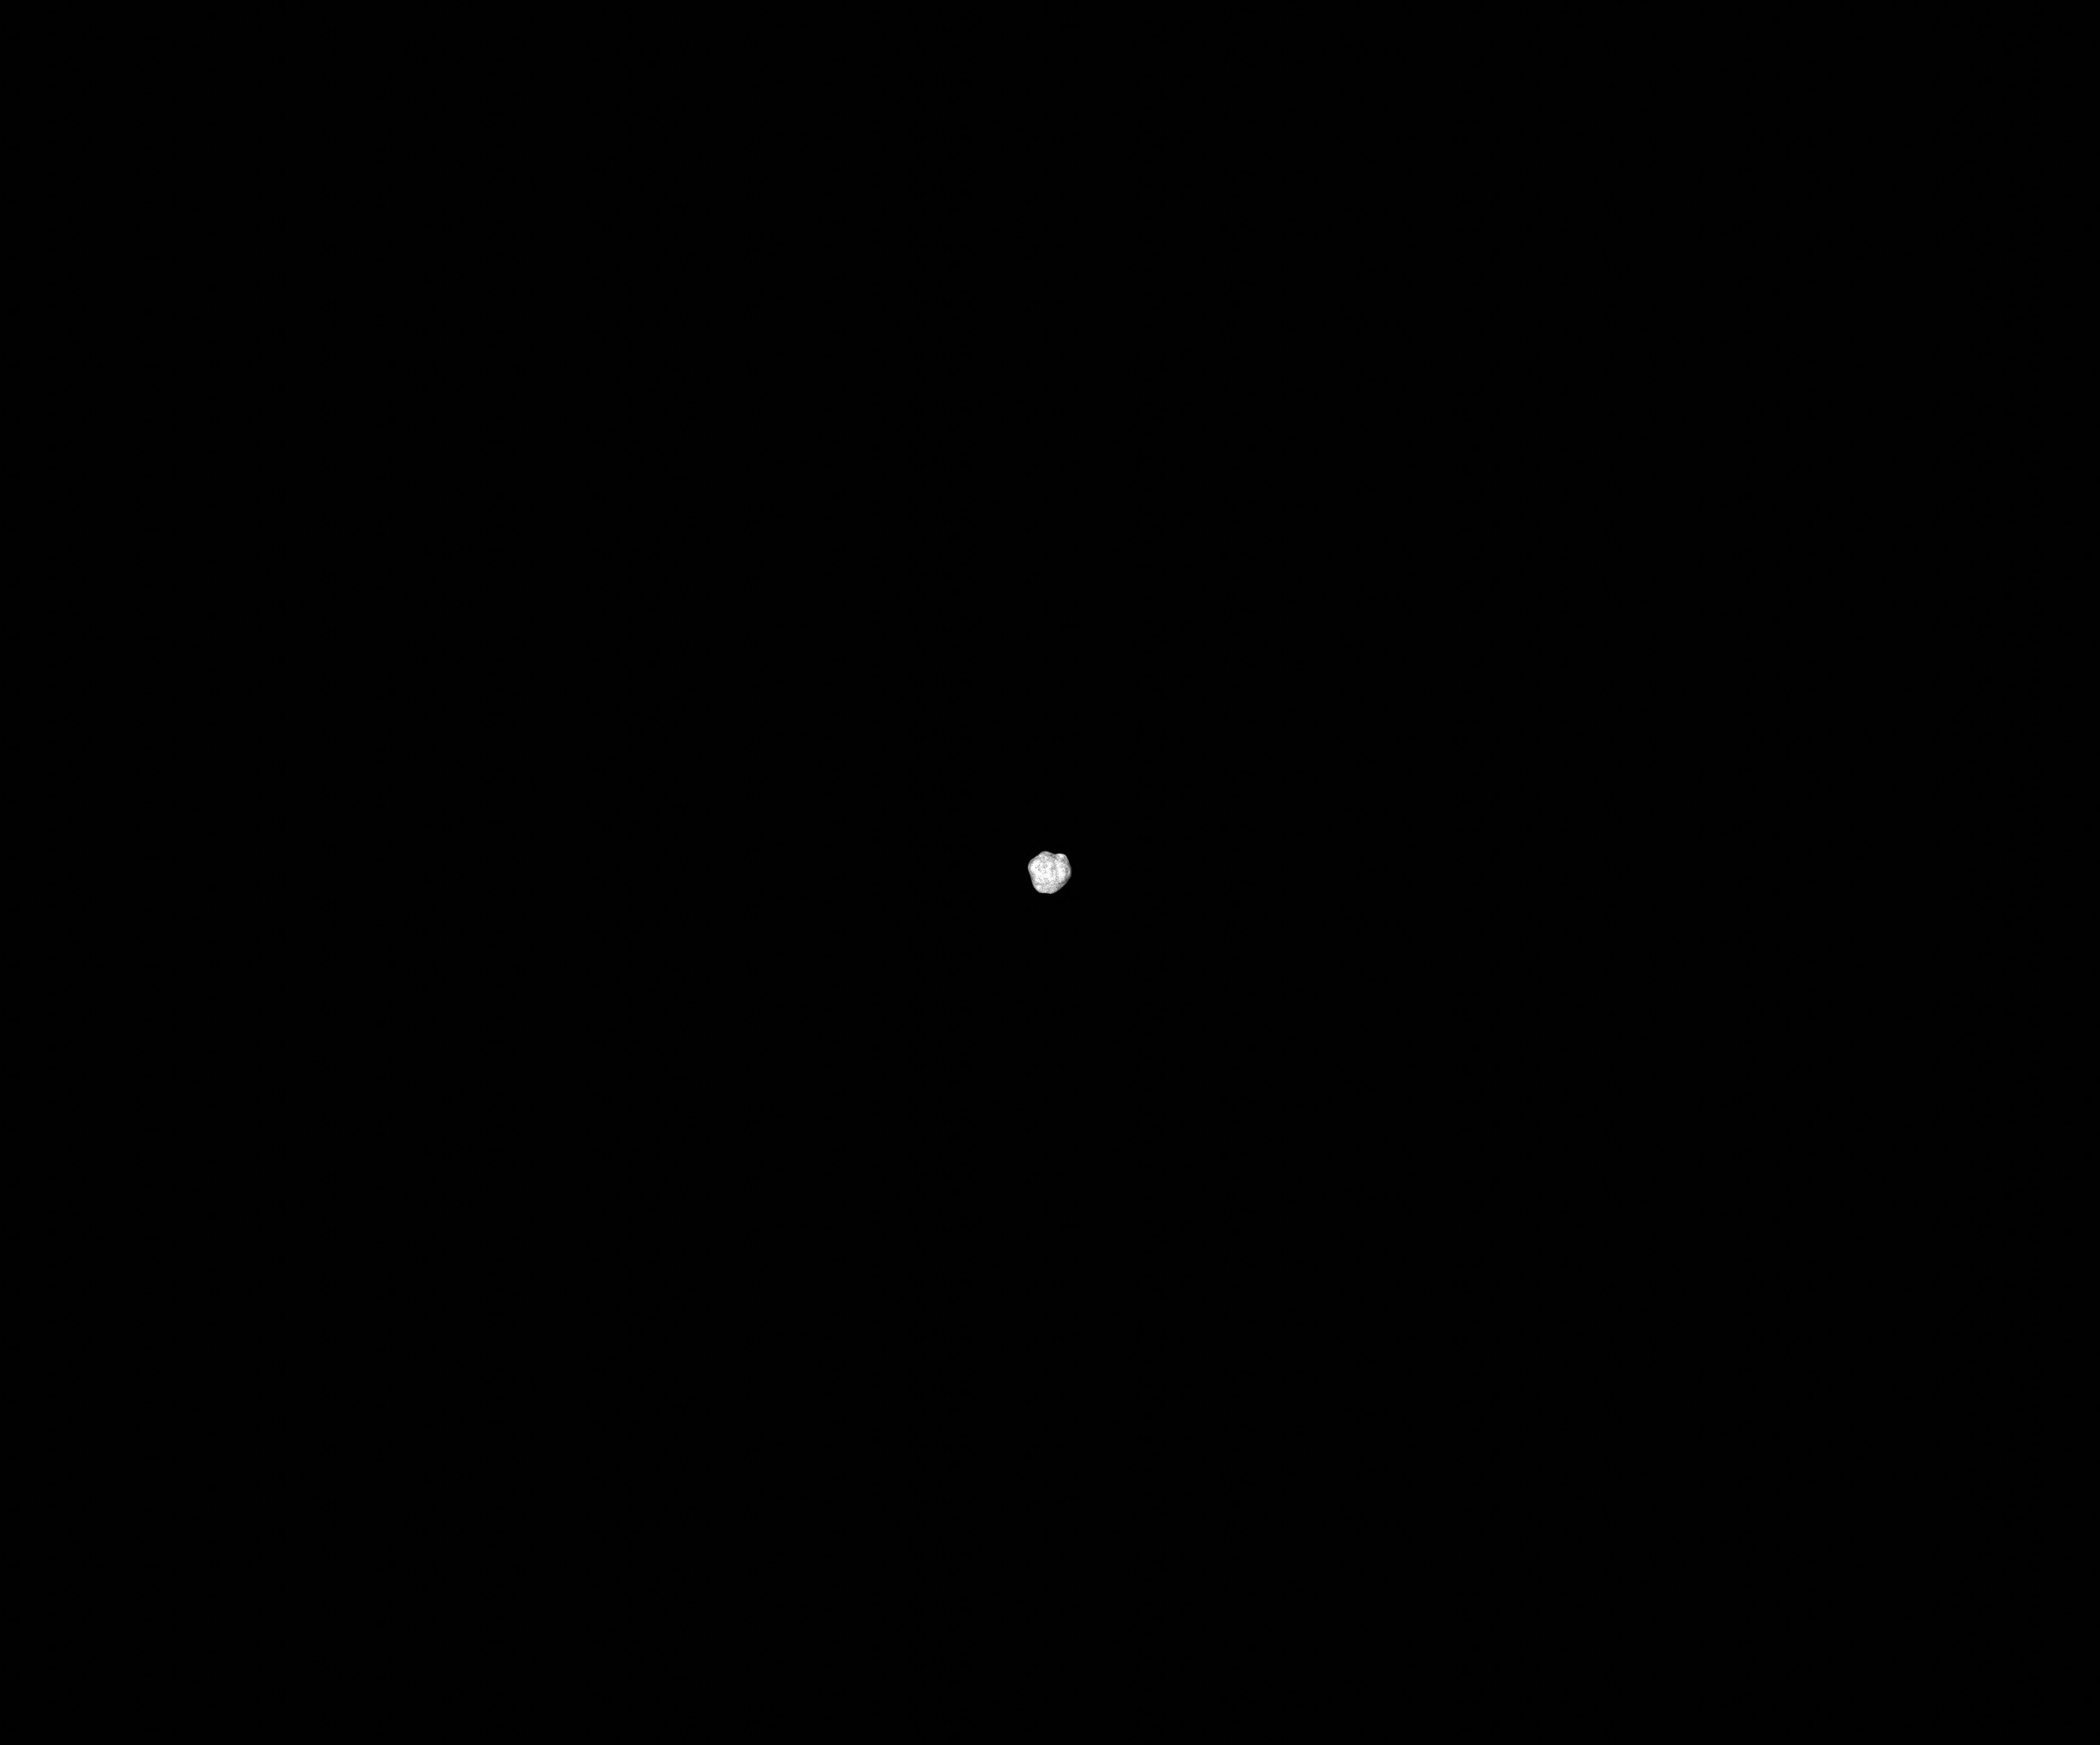
\includegraphics[height=8cm]{doc/thesis/0_figures/cv_skimage/SssbConstDist_2017-08-15T115851-679000.jpg}
    \end{center}
    \caption{SssbConstDist image used in benchmark.}
    \label{fig:bm_sssbconstdist}
\end{figure}

\begin{figure}[htb]
    \begin{center}
        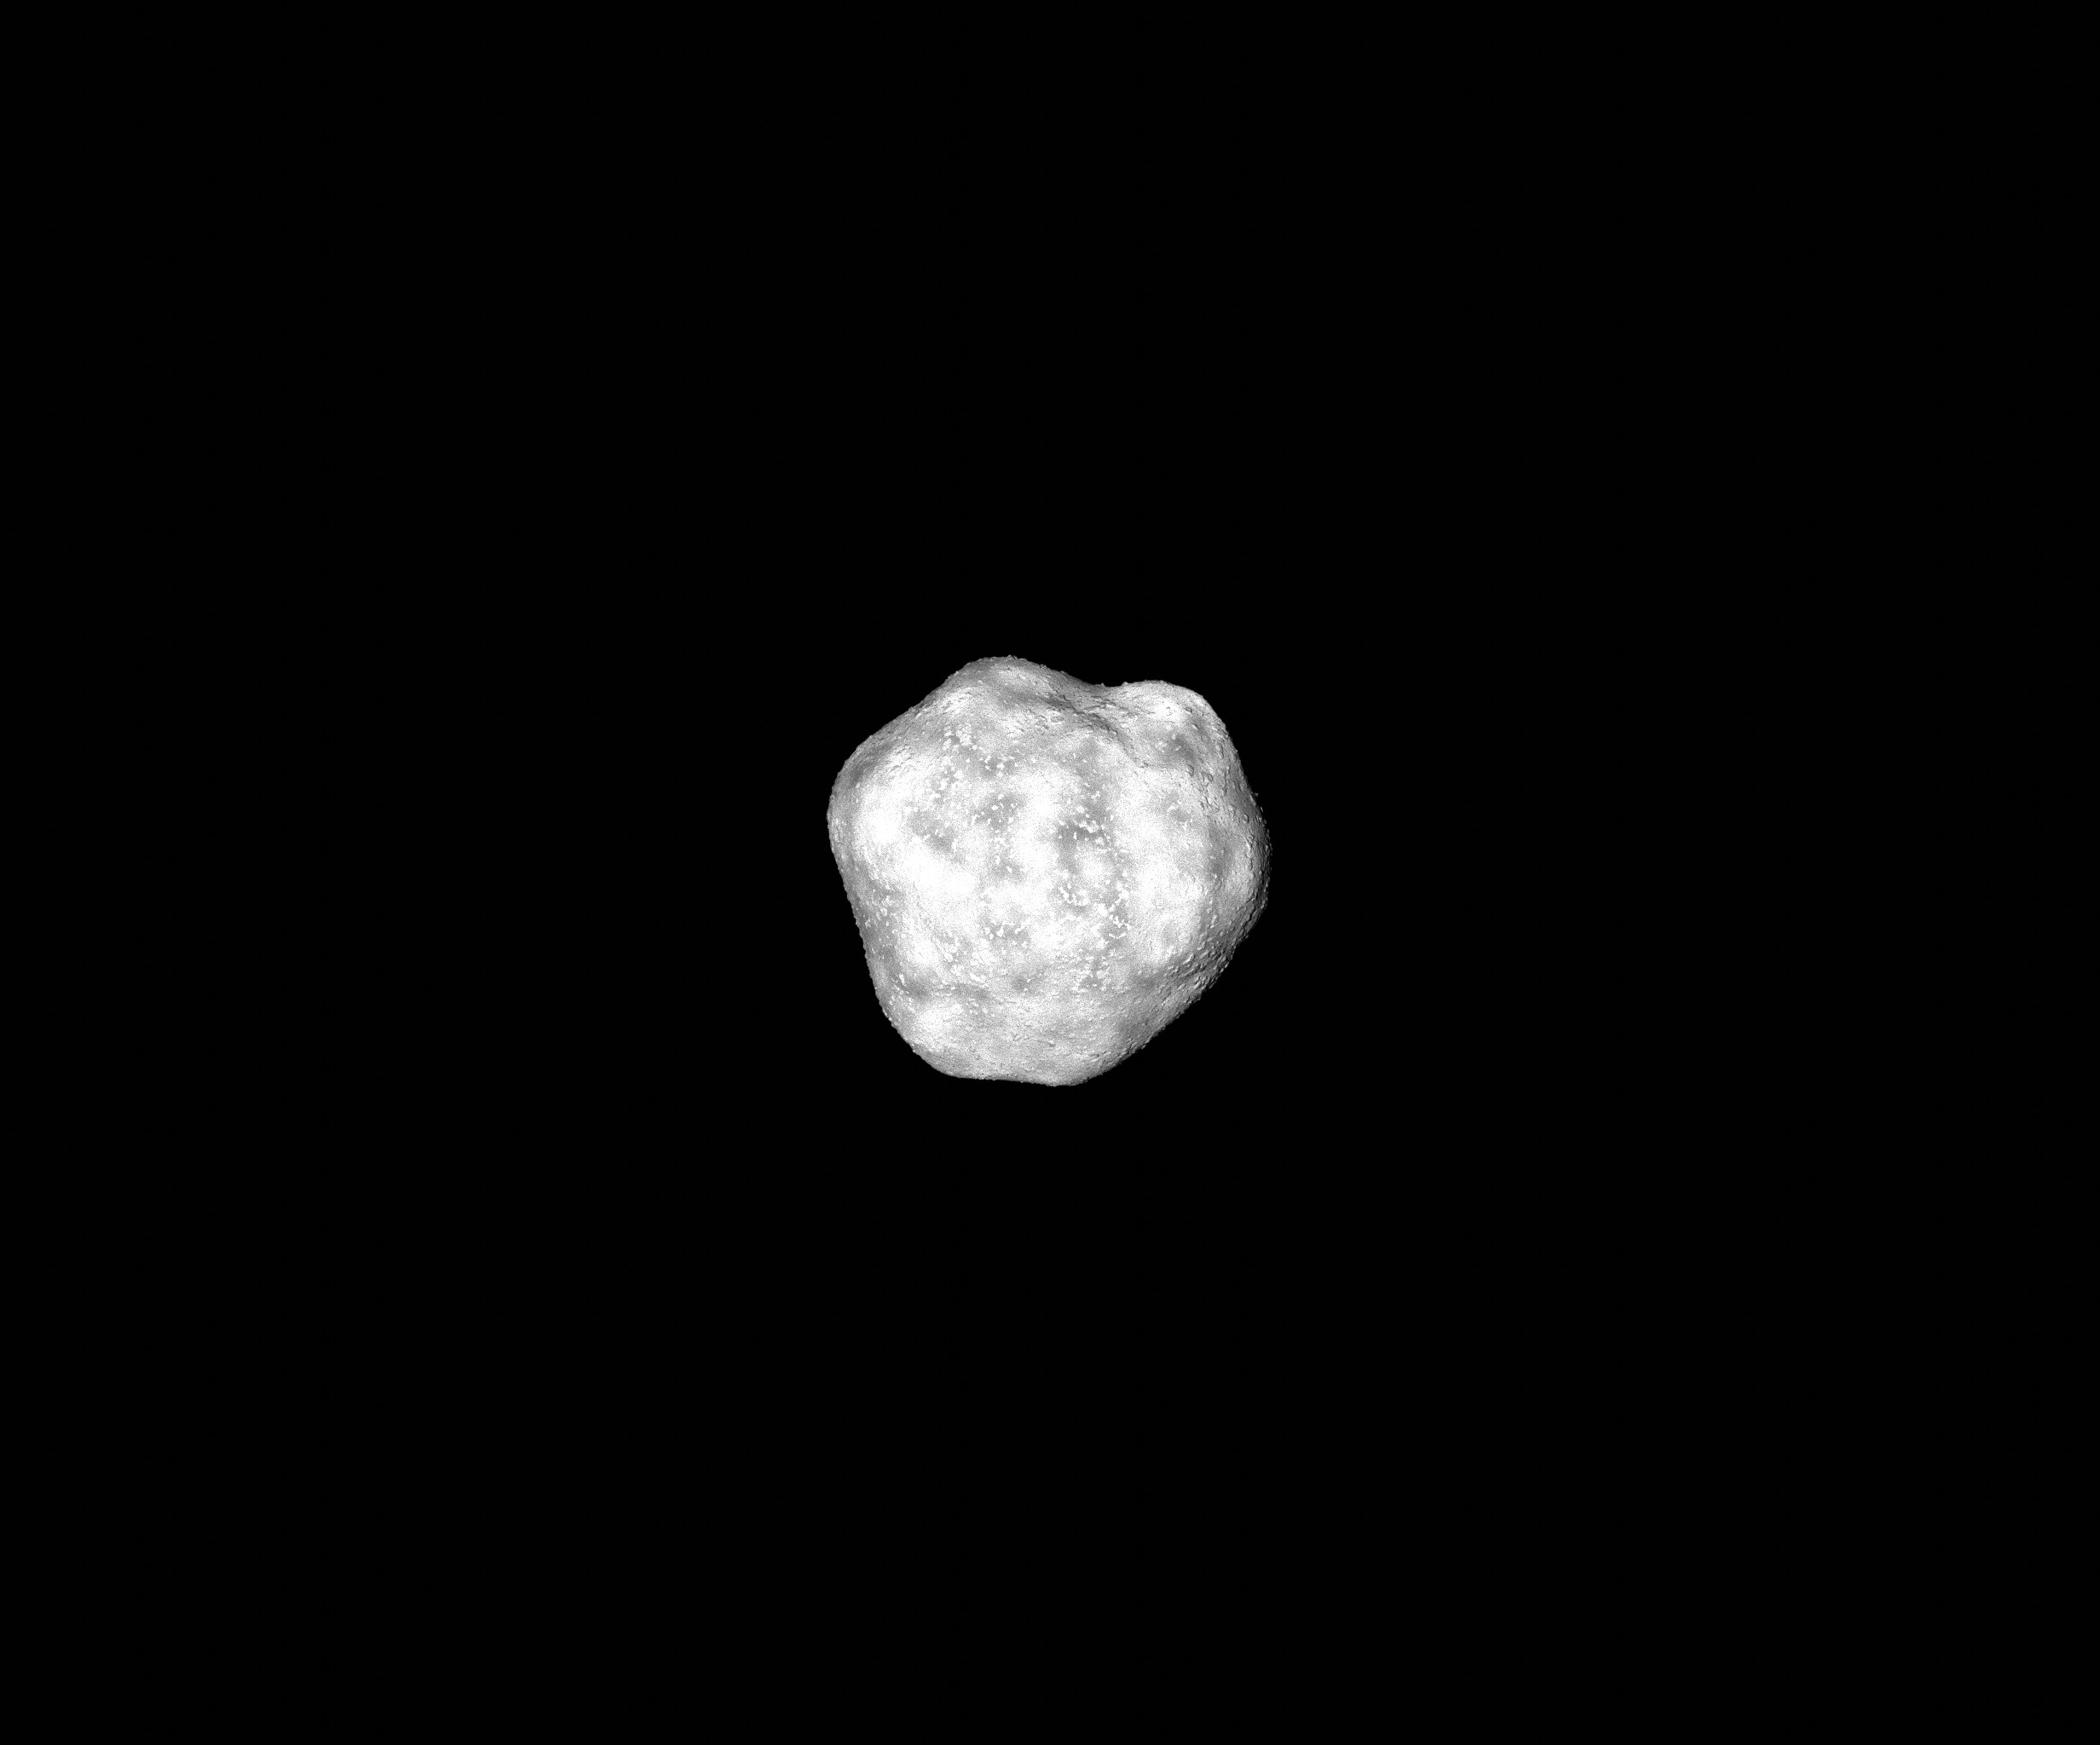
\includegraphics[height=8cm]{doc/thesis/0_figures/cv_skimage/SssbOnly_2017-08-15T115851-679000.jpg}
    \end{center}
    \caption{SssbOnly image used in benchmark.}
    \label{fig:bm_sssbonly}
\end{figure}

\begin{figure}[htb]
    \begin{center}
        
\includegraphics[height=8cm]{doc/thesis/0_figures/cv_skimage/Stars_2017-08-15T115841-334000.png}
    \end{center}
    \caption{Stars1 image used in benchmark. The image is based on 1804 stars.}
    \label{fig:bm_stars1}
\end{figure}

\begin{figure}[htb]
    \begin{center}
        
\includegraphics[height=8cm]{doc/thesis/0_figures/cv_skimage/Stars_2017-08-15T115857-362000.png}
    \end{center}
    \caption{Stars2 image used in benchmark. The image is based on 51338 stars.}
    \label{fig:bm_stars2}
\end{figure}

Figures \ref{fig:bm_light_ref} through \ref{fig:bm_stars2} are the images used in the benchmark. Their names are given in the respective caption.

\begin{figure}[htb]
    \begin{center}
        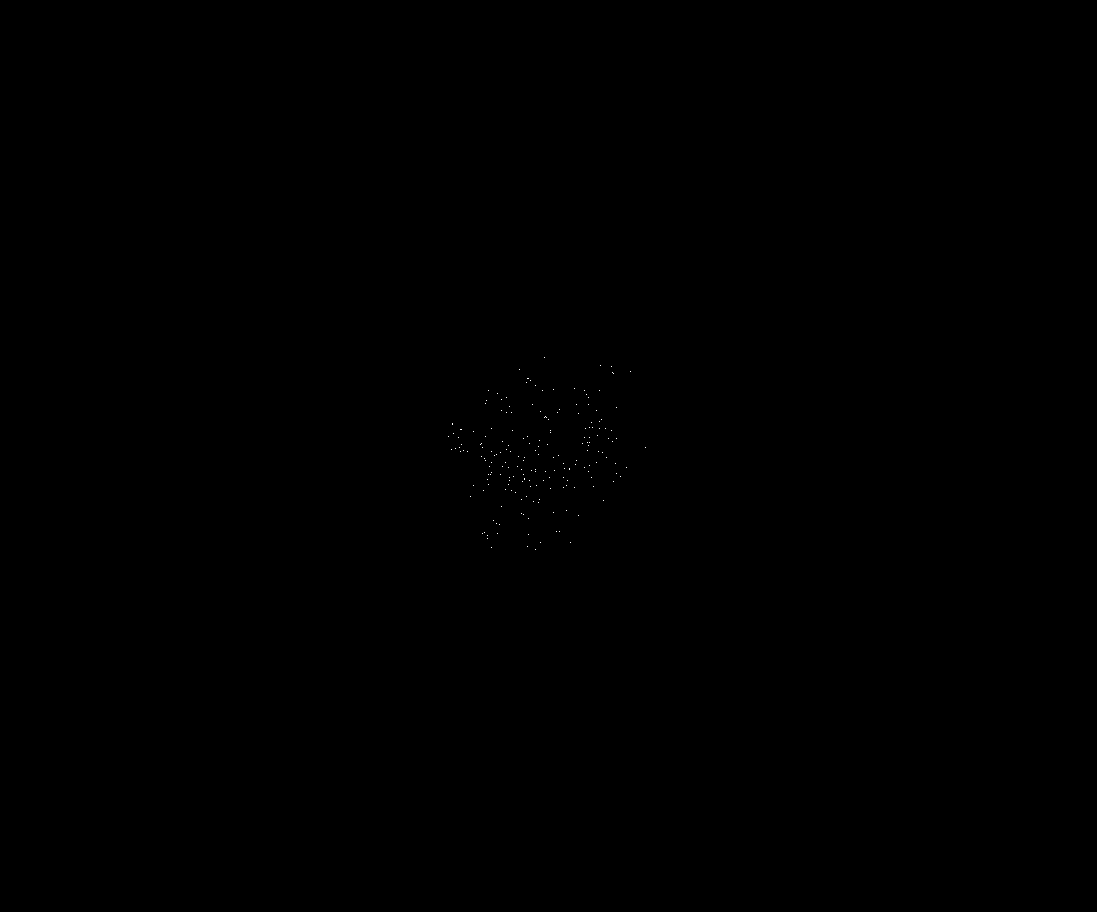
\includegraphics[height=8cm]{doc/thesis/0_figures/cv_skimage/diff_laptop.png}
    \end{center}
    \caption{Difference between \gls{skimage} and OpenCV Gaussian filtered SssbOnly image of the laptop.}
    \label{fig:bm_diff_laptop}
\end{figure}

\begin{figure}[htb]
    \begin{center}
        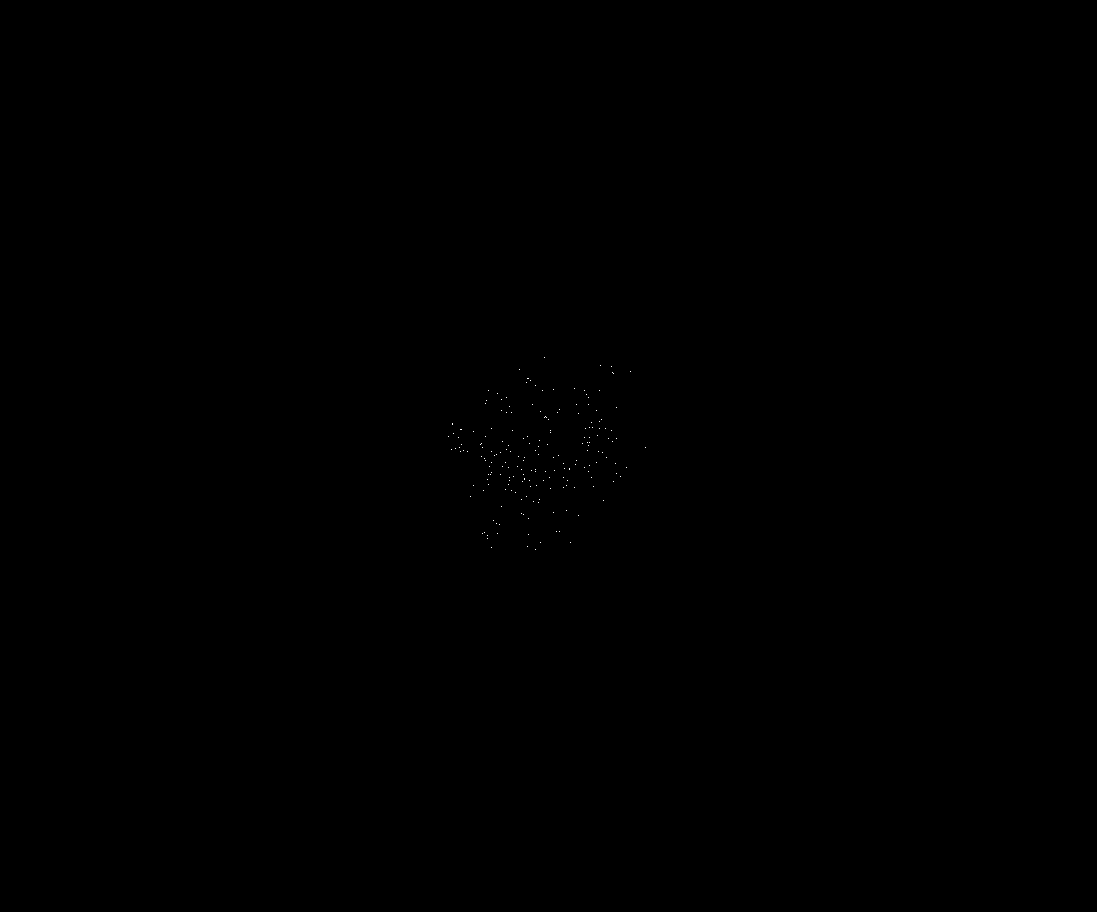
\includegraphics[height=8cm]{doc/thesis/0_figures/cv_skimage/diff_workstation.png}
    \end{center}
    \caption{Difference between \gls{skimage} and OpenCV Gaussian filtered SssbOnly image of the workstation.}
    \label{fig:bm_diff_workstation}
\end{figure}

Figures \ref{fig:bm_diff_laptop} and \ref{fig:bm_diff_workstation} show the difference of the SssbOnly image from the benchmark on the two different computers. Only a small fraction of pixels differ. As discussed previously, the maximum absolute difference is on the order of \SI{1e-6}{}, corresponding to the brightest point in each image. 

\end{document}
